% /*
% 		    GNU GENERAL PUBLIC LICENSE
% 		       Version 2, June 1991
% 
%  Copyright (C) 1989, 1991 Free Software Foundation, Inc.
%                        59 Temple Place, Suite 330, Boston, MA  02111-1307  USA
%  Everyone is permitted to copy and distribute verbatim copies
%  of this license document, but changing it is not allowed.
% 
% 			    Preamble
% 
%   The licenses for most software are designed to take away your
% freedom to share and change it.  By contrast, the GNU General Public
% License is intended to guarantee your freedom to share and change free
% software--to make sure the software is free for all its users.  This
% General Public License applies to most of the Free Software
% Foundation's software and to any other program whose authors commit to
% using it.  (Some other Free Software Foundation software is covered by
% the GNU Library General Public License instead.)  You can apply it to
% your programs, too.
% 
%   When we speak of free software, we are referring to freedom, not
% price.  Our General Public Licenses are designed to make sure that you
% have the freedom to distribute copies of free software (and charge for
% this service if you wish), that you receive source code or can get it
% if you want it, that you can change the software or use pieces of it
% in new free programs; and that you know you can do these things.
% 
%   To protect your rights, we need to make restrictions that forbid
% anyone to deny you these rights or to ask you to surrender the rights.
% These restrictions translate to certain responsibilities for you if you
% distribute copies of the software, or if you modify it.
% 
%   For example, if you distribute copies of such a program, whether
% gratis or for a fee, you must give the recipients all the rights that
% you have.  You must make sure that they, too, receive or can get the
% source code.  And you must show them these terms so they know their
% rights.
% 
%   We protect your rights with two steps: (1) copyright the software, and
% (2) offer you this license which gives you legal permission to copy,
% distribute and/or modify the software.
% 
%   Also, for each author's protection and ours, we want to make certain
% that everyone understands that there is no warranty for this free
% software.  If the software is modified by someone else and passed on, we
% want its recipients to know that what they have is not the original, so
% that any problems introduced by others will not reflect on the original
% authors' reputations.
% 
%   Finally, any free program is threatened constantly by software
% patents.  We wish to avoid the danger that redistributors of a free
% program will individually obtain patent licenses, in effect making the
% program proprietary.  To prevent this, we have made it clear that any
% patent must be licensed for everyone's free use or not licensed at all.
% 
%   The precise terms and conditions for copying, distribution and
% modification follow.
% 
% 		    GNU GENERAL PUBLIC LICENSE
%    TERMS AND CONDITIONS FOR COPYING, DISTRIBUTION AND MODIFICATION
% 
%   0. This License applies to any program or other work which contains
% a notice placed by the copyright holder saying it may be distributed
% under the terms of this General Public License.  The "Program", below,
% refers to any such program or work, and a "work based on the Program"
% means either the Program or any derivative work under copyright law:
% that is to say, a work containing the Program or a portion of it,
% either verbatim or with modifications and/or translated into another
% language.  (Hereinafter, translation is included without limitation in
% the term "modification".)  Each licensee is addressed as "you".
% 
% Activities other than copying, distribution and modification are not
% covered by this License; they are outside its scope.  The act of
% running the Program is not restricted, and the output from the Program
% is covered only if its contents constitute a work based on the
% Program (independent of having been made by running the Program).
% Whether that is true depends on what the Program does.
% 
%   1. You may copy and distribute verbatim copies of the Program's
% source code as you receive it, in any medium, provided that you
% conspicuously and appropriately publish on each copy an appropriate
% copyright notice and disclaimer of warranty; keep intact all the
% notices that refer to this License and to the absence of any warranty;
% and give any other recipients of the Program a copy of this License
% along with the Program.
% 
% You may charge a fee for the physical act of transferring a copy, and
% you may at your option offer warranty protection in exchange for a fee.
% 
%   2. You may modify your copy or copies of the Program or any portion
% of it, thus forming a work based on the Program, and copy and
% distribute such modifications or work under the terms of Section 1
% above, provided that you also meet all of these conditions:
% 
%     a) You must cause the modified files to carry prominent notices
%     stating that you changed the files and the date of any change.
% 
%     b) You must cause any work that you distribute or publish, that in
%     whole or in part contains or is derived from the Program or any
%     part thereof, to be licensed as a whole at no charge to all third
%     parties under the terms of this License.
% 
%     c) If the modified program normally reads commands interactively
%     when run, you must cause it, when started running for such
%     interactive use in the most ordinary way, to print or display an
%     announcement including an appropriate copyright notice and a
%     notice that there is no warranty (or else, saying that you provide
%     a warranty) and that users may redistribute the program under
%     these conditions, and telling the user how to view a copy of this
%     License.  (Exception: if the Program itself is interactive but
%     does not normally print such an announcement, your work based on
%     the Program is not required to print an announcement.)
% 
% These requirements apply to the modified work as a whole.  If
% identifiable sections of that work are not derived from the Program,
% and can be reasonably considered independent and separate works in
% themselves, then this License, and its terms, do not apply to those
% sections when you distribute them as separate works.  But when you
% distribute the same sections as part of a whole which is a work based
% on the Program, the distribution of the whole must be on the terms of
% this License, whose permissions for other licensees extend to the
% entire whole, and thus to each and every part regardless of who wrote it.
% 
% Thus, it is not the intent of this section to claim rights or contest
% your rights to work written entirely by you; rather, the intent is to
% exercise the right to control the distribution of derivative or
% collective works based on the Program.
% 
% In addition, mere aggregation of another work not based on the Program
% with the Program (or with a work based on the Program) on a volume of
% a storage or distribution medium does not bring the other work under
% the scope of this License.
% 
%   3. You may copy and distribute the Program (or a work based on it,
% under Section 2) in object code or executable form under the terms of
% Sections 1 and 2 above provided that you also do one of the following:
% 
%     a) Accompany it with the complete corresponding machine-readable
%     source code, which must be distributed under the terms of Sections
%     1 and 2 above on a medium customarily used for software interchange; or,
% 
%     b) Accompany it with a written offer, valid for at least three
%     years, to give any third party, for a charge no more than your
%     cost of physically performing source distribution, a complete
%     machine-readable copy of the corresponding source code, to be
%     distributed under the terms of Sections 1 and 2 above on a medium
%     customarily used for software interchange; or,
% 
%     c) Accompany it with the information you received as to the offer
%     to distribute corresponding source code.  (This alternative is
%     allowed only for noncommercial distribution and only if you
%     received the program in object code or executable form with such
%     an offer, in accord with Subsection b above.)
% 
% The source code for a work means the preferred form of the work for
% making modifications to it.  For an executable work, complete source
% code means all the source code for all modules it contains, plus any
% associated interface definition files, plus the scripts used to
% control compilation and installation of the executable.  However, as a
% special exception, the source code distributed need not include
% anything that is normally distributed (in either source or binary
% form) with the major components (compiler, kernel, and so on) of the
% operating system on which the executable runs, unless that component
% itself accompanies the executable.
% 
% If distribution of executable or object code is made by offering
% access to copy from a designated place, then offering equivalent
% access to copy the source code from the same place counts as
% distribution of the source code, even though third parties are not
% compelled to copy the source along with the object code.
% 
%   4. You may not copy, modify, sublicense, or distribute the Program
% except as expressly provided under this License.  Any attempt
% otherwise to copy, modify, sublicense or distribute the Program is
% void, and will automatically terminate your rights under this License.
% However, parties who have received copies, or rights, from you under
% this License will not have their licenses terminated so long as such
% parties remain in full compliance.
% 
%   5. You are not required to accept this License, since you have not
% signed it.  However, nothing else grants you permission to modify or
% distribute the Program or its derivative works.  These actions are
% prohibited by law if you do not accept this License.  Therefore, by
% modifying or distributing the Program (or any work based on the
% Program), you indicate your acceptance of this License to do so, and
% all its terms and conditions for copying, distributing or modifying
% the Program or works based on it.
% 
%   6. Each time you redistribute the Program (or any work based on the
% Program), the recipient automatically receives a license from the
% original licensor to copy, distribute or modify the Program subject to
% these terms and conditions.  You may not impose any further
% restrictions on the recipients' exercise of the rights granted herein.
% You are not responsible for enforcing compliance by third parties to
% this License.
% 
%   7. If, as a consequence of a court judgment or allegation of patent
% infringement or for any other reason (not limited to patent issues),
% conditions are imposed on you (whether by court order, agreement or
% otherwise) that contradict the conditions of this License, they do not
% excuse you from the conditions of this License.  If you cannot
% distribute so as to satisfy simultaneously your obligations under this
% License and any other pertinent obligations, then as a consequence you
% may not distribute the Program at all.  For example, if a patent
% license would not permit royalty-free redistribution of the Program by
% all those who receive copies directly or indirectly through you, then
% the only way you could satisfy both it and this License would be to
% refrain entirely from distribution of the Program.
% 
% If any portion of this section is held invalid or unenforceable under
% any particular circumstance, the balance of the section is intended to
% apply and the section as a whole is intended to apply in other
% circumstances.
% 
% It is not the purpose of this section to induce you to infringe any
% patents or other property right claims or to contest validity of any
% such claims; this section has the sole purpose of protecting the
% integrity of the free software distribution system, which is
% implemented by public license practices.  Many people have made
% generous contributions to the wide range of software distributed
% through that system in reliance on consistent application of that
% system; it is up to the author/donor to decide if he or she is willing
% to distribute software through any other system and a licensee cannot
% impose that choice.
% 
% This section is intended to make thoroughly clear what is believed to
% be a consequence of the rest of this License.
% 
%   8. If the distribution and/or use of the Program is restricted in
% certain countries either by patents or by copyrighted interfaces, the
% original copyright holder who places the Program under this License
% may add an explicit geographical distribution limitation excluding
% those countries, so that distribution is permitted only in or among
% countries not thus excluded.  In such case, this License incorporates
% the limitation as if written in the body of this License.
% 
%   9. The Free Software Foundation may publish revised and/or new versions of the General Public License from time to time.  Such new versions will be similar in spirit to the present version, but may differ in detail to address new problems or concerns.
% 
% Each version is given a distinguishing version number.  If the Program
% specifies a version number of this License which applies to it and "any
% later version", you have the option of following the terms and conditions 
% either of that version or of any later version published by the Free Software 
% Foundation.  If the Program does not specify a version number of this License,
%  you may choose any version ever published by the Free Software Foundation.
% 
%   10. If you wish to incorporate parts of the Program into other free
% programs whose distribution conditions are different, write to the author to 
% ask for permission.  For software which is copyrighted by the Free Software 
% Foundation, write to the Free Software Foundation; we sometimes make 
% exceptions for this.  Our decision will be guided by the two goals of 
% preserving the free status of all derivatives of our free software and of 
% promoting the sharing and reuse of software generally.
% 
% 			    NO WARRANTY
% 
%   11. BECAUSE THE PROGRAM IS LICENSED FREE OF CHARGE, THERE IS NO WARRANTY FOR
% THE PROGRAM, TO THE EXTENT PERMITTED BY APPLICABLE LAW.  EXCEPT WHEN 
% OTHERWISE STATED IN WRITING THE COPYRIGHT HOLDERS AND/OR OTHER PARTIES PROVIDE 
% THE PROGRAM "AS IS" WITHOUT WARRANTY OF ANY KIND, EITHER EXPRESSED OR IMPLIED, 
% INCLUDING, BUT NOT LIMITED TO, THE IMPLIED WARRANTIES OF MERCHANTABILITY AND 
% FITNESS FOR A PARTICULAR PURPOSE.  THE ENTIRE RISK AS TO THE QUALITY AND 
% PERFORMANCE OF THE PROGRAM IS WITH YOU.  SHOULD THE PROGRAM PROVE DEFECTIVE, 
% YOU ASSUME THE COST OF ALL NECESSARY SERVICING, REPAIR OR CORRECTION.
% 
%   12. IN NO EVENT UNLESS REQUIRED BY APPLICABLE LAW OR AGREED TO IN WRITING 
% WILL ANY COPYRIGHT HOLDER, OR ANY OTHER PARTY WHO MAY MODIFY AND/OR 
% REDISTRIBUTE THE PROGRAM AS PERMITTED ABOVE, BE LIABLE TO YOU FOR DAMAGES, 
% INCLUDING ANY GENERAL, SPECIAL, INCIDENTAL OR CONSEQUENTIAL DAMAGES ARISING 
% OUT OF THE USE OR INABILITY TO USE THE PROGRAM (INCLUDING BUT NOT LIMITED TO 
% LOSS OF DATA OR DATA BEING RENDERED INACCURATE OR LOSSES SUSTAINED BY YOU OR 
% THIRD PARTIES OR A FAILURE OF THE PROGRAM TO OPERATE WITH ANY OTHER PROGRAMS), 
% EVEN IF SUCH HOLDER OR OTHER PARTY HAS BEEN ADVISED OF THE POSSIBILITY OF SUCH 
% DAMAGES.
% 
% 		     END OF TERMS AND CONDITIONS
% */
      \htmlmenu{4}

\s{Getting Started}{GettingStarted}

   This section helps new users get started with the
   readout software.  This section describes:
   \begin{itemize}
      \item How to obtain a copy of the files you will need
	    to tailor the readout software to your experiment
	    (Described in 
	    \link{Obtaining the Readout skeleton}[
	       Section \ref{ss:Obtaining}]{ss:Obtaining}).
      \item How to modify this skeleton to meet the needs of
	    your experiment (Described in
	    \link{Modifying the Readout Skeleton}[
	       Section \ref{ss:Modifying}]{ss:Modifying}).
      \item How to add scaler readout to your skeleton (described
	 in \link{Setting up scaler readout}{ss:scalers}
      \item How to compile a tailored version of the readout
	    software once you have finished your modifications
	    (Described in 
	    \link{Compiling your Readout software}[
	       Section \ref{ss:Compiling}]{ss:Compiling}).
      \item How to set up your trigger electronics and 
	    the computer busy lockout (Described in:
	    \link{Setting up the electronics}[
	       Section \ref{ss:Electronics}]{ss:Electronics}
     \item How to run the readout program you have built.
	    (Described in :
	    \link{Running your readout software}[
	       Section \ref{ss:Running}]{ss:Running}).
 	    
   \end{itemize}

   These sections roughly reflect order in which you should
   do things with the Readout software.

   Throughout this document we'll follow the conventions:
   \begin{itemize}
      \item The software is installed relative to an
	 environment variable: DAQROOT
      \item Things typed by the computer will be \computer{italicized}
      \item Things you must type will be in \human{bold}.
   \end{itemize}

   \subs{Obtaining the Readout skeleton}{Obtaining}
   
   The readout skeleton is an application framework.  
   Application frameworks are harnesses that take care of all
   of the flow control of the application and leave you with 
   the task of filling in application specific code only.  
   In the case of Readout, we also provide a sample skeleton
   program that you can modifiy as required by your experimental
   application.
   
   The first step in this modification process is to obtain a
   clean copy of the skeleton software.   Unless there is a
   very good reason to do otherwise, you should always start
   with fresh skeleton software so that you are getting the
   latest, most debugged software.  See
   \link{Tailoring dos and don'ts}[
      Section \ref{ss:Readoutstyleguide}]{ss:Readoutstyleguide} for some
   coding style suggestions that will make it easier to upgrade
   to newer skeleton versions.
   
   To get a copy of the skeleton software:
   \begin{example}
   \computer{$<>$ }\human{mkdir MyReadout }
   \computer{$<>$ }\human{cd MyReadout }
   \computer{$<$MyReadout$>$ } \human{cp \$DAQROOT/pReadoutSkeleton/* . }
   
   \end{example}

   These commands create a new directory {\bf MyReadout}, and
   copy the following files into it:
   \begin{description}
      \item{Skeleton.cpp} The source C$++$ file that you will
	 need to modify to meet your readout requirements.
	 (See 
	 \link{Modifying the Readout Skeleton}[
	 Section \ref{ss:Modifying}]{ss:Modifying}).
      \item{CTraditionalEventSegment.cpp}  The C$++$ source file that
	  contains the traditional event segment implementation.  You will need
	  to build and link this file if you are using traditional event
	  segments (see  \link{Incorporating ``traditional'' readout software}[
	Section {sss:traditional}]{sss:traditional} for more information
	about traditional readout segments).
      \item {CTraditionalScalerReadout.cpp}  The C$++$ source file that
	  contains the traditional scaler readout implementation.  You
	  will need to build and link this file if you are using traditional
	  scaler readout (see \link{Traditional scaler readout}[
	 Section \ref{sss:straditional}]{sss:straditional} for more 
	information about traditional scaler readout).
      \item{Makefile}  An input file to the make utility that
	 you may need to modify if you want make to compile
	 additional C$++$ source modules and build them into
	 your Readout program.
	 \link{Compiling your readout software}[
	    Section \ref{ss:Compiling}]{ss:Compiling}
   \end{description}

   \subs{Modifiying the Readout skeleton}{Modifying}
   
      The source file {MyReadout.cpp} is defines and
      makes an instance of a class that is derived from 
      CReadoutMain.  Member functions of the object 
      created will be called at well defined points in the
      startup of the Readout program.  A complete list of
      the entry points, when they are called and what they can
      be used for is given in \link{Tailoring the software}[
      Section \ref{s:Readouttailoring}]{s:Readouttailoring}
      
      In this section, we'll look at the simplest modifications
      needed to get an experiment read out.  We will also look
      at how to incorporate readout code from the old readout 
      program
      (referred to here as the ``traditional'' readout system)
      into the NSCL readout software.
      
      Continue reading with one of the choices below 
      depending on how
      you want to structure your readout software:
      
      \begin{itemize}
	 \item \link{Suggested way to structure your readout}[
	    continue reading at Section 
	    \ref{sss:newreadout}]{sss:newreadout}
	 \item \link{Incorporating ``traditional'' readout software}[
	    continue reading at Section 
	    \ref{sss:traditional}]{sss:traditional}
      \end{itemize}
      

      \subsubs{How to structure your readout}{newreadout}
      
      Before describing how to modify the readout software, it is 
      important to understand how the readout software organizes
      the readout.  There are two organizations to consider; The 
      logical way in which you programmatically desribe the 
      readout to the software, and the physical layout of the
      corresponding event in the event buffer.
      
      The new NSCL readout software logically 
      organizes events in chunks. 
      Each chunk is
      called an {\em Event Segment}.  The framework supports three
      types of event segements:
      \begin{description}
	 \item{Simple}  Described by objects that are
	    derived from the class CEventSegment.
	 \item{Compound} Described by a CCompoundEventSegment
	    object that has had other event segments (both simple
	    and compound) inserted into it.
	 \item{Traditional}  A single object of type 
	    CTraditionalEventSegment can be incorporated in your
	    readout.  
	    \link{Incorporating ``traditional'' readout software}[
	    , Section \ref{sss:traditional}]{sss:traditional} 
	    describes how to use this mechanism to incorporate
	    legacy readout software.  It is also possible to
	    put the single tradtional readout segement into
	    a compound readout segement and in this way merge it
	    with more modern readout software.
      \end{description}
      
   The physical structure of an event is essentially up to the
   requirements of an experiment.  The overall structure of
   an event buffer is described in \link{Event Data Buffers}[
      (Section \ref{ss:EventBufferFormat}).]{ss:EventBufferFormat}
   We recommend that you structure your physical readout in 
   documented packets.  The examples in this section will show
   how to do this, however complete information about documented
   packets and what they give you is in 
   \link{Documenting event segment packet types}[ (Section
      \ref{ss:Packetdocs}).]{ss:Packetdocs}

   Let's now look at how to specify what is read out.  To
   create a simple readout, you will need to:
   \begin{itemize}
      \item Create a class that inherits from CEventSegment, call it
		MyEventSegment
      \item Fill in the the Initialize, Clear and Read member functions of
		this new class to initialize, clear and read the devices you
		want to read.
      \item In MyExperiment.cpp, locate the implementation of 
		SetupReadout and the comment:
		\begin{verbatim}
		// Insert your code below this comment.
		\end{verbatim}
		Add the line:
		\begin{verbatim}
		rExperiment.AddEventSegment(new MyEventSegment);
		\end{verbatim}
      \item Compile your readout as described in 
		\link{Compiling your readout software}[
		, Section \ref{ss:Compiling}]{ss:Compiling}.
   \end{itemize}


   To use Compound Event segments:
   \begin{itemize}
      \item Create several classes that inherit from CEventSegment
	 for example Myseg1, Myseg2.
      \item Fill in the Initialize, Clear and Read member
	 functions for all of your segments.
      \item In MyExperiment.cpp, locate the implementation of 
	    SetupReadout and the comment:
	    \begin{verbatim}
	    // Insert your code below this comment.
	    \end{verbatim}
	    Add the lines:
	    \begin{verbatim}
	    CCompoundEventSegment* p = new CCompoundEventSegment;
	    p->AddSegment(new Myseg1);
	    p->AddSegment(new Myseg2);
	    rExperiment.AddEventSegment(p);
	    \end{verbatim}
      \item Compile your readout as described in 
	    \link{Compiling your readout software}[
	    , Section \ref{ss:Compiling}]{ss:Compiling}.   
   \end{itemize}
   
      Note that you may also use compound event segments to build
   up a hierarchical organization of the readout system.  To do this,
   simply create compound event objects and embed them in other compound
   event objects.

  \subsubs{Incorporating ``traditional'' readout software}{traditional}
   Since the NSCL Data Acquisition system has run for several years with
   a prototoype readout skeleton, there is quite a large body of existing
   readout code.  We'll refer to this code as ``traditional'' readout software.
   The current readout software supports incorporating a single traditional
   readout skeleton in the experiment readout.  For simple experiments this 
   will be sufficient, however for complex experiments, that merge data from
   several apparati, you should consider porting your readout to the object
   oriented readout scheme described in \link{How to Structure Your Readout}[
   , Section \ref{sss:newreadout}]{sss:newreadout}.
   
   Traditional readout support is done by wrapping the skeleton of the traditional
   readout software in an object of type: CTraditionalEventSegment. To do this in your readout:
   \begin{itemize}
      \item Obtain the readout skeleton as described in 
      \link{Obtaining the Readout skeleton}[ (Section \ref{ss:Obtaining})]
      {ss:Obtaining}.
      \item Copy the skeleton.cpp and all headers and other source files you
	 wrote to your readout working directory.  Do not copy ReadoutMain.cpp.
      \item Modify your Makefile so that it will build skeleton.o and any other 
	 object modules your software needs.
      \item In MyExperiment.cpp, locate the implementation of 
	    SetupReadout and the comment:
	    \begin{verbatim}
	    // Insert your code below this comment.
	    \end{verbatim}
	    Add the line:
	    \begin{verbatim}
	    rExperiment.AddEventSegment(new CTraditionalEventSegment);
	    \end{verbatim}
   \end{itemize}
   \subs{Setting up scaler readout}{scalers}
      The readout skeleton supports periodic readout of run time scalers.  
      At the end of each scaler interval, scalers are read and cleared. 
      Thus the scaler data in the data buffers is incremental.  Using
      incremental scalers means that you do not generally have to worry 
      about scalers overflowing, however reading scalers incrementally  can
      not be done atomically so there will be some lost scaler counts.
      The scaler busy output can be used to approximate the severity of this
      effect and correct for it.  See 
      \link{Setting up the electronics}[ 
      (Section \ref{ss:Electronics})]{ss:Electronics}.
      
      As is the case for event readout, two types of scaler readout are
      supported, a composite scheme and a traditional scheme:
      
      The structured scaler readout scheme allows you to structure
      scalers in to banks, and insert scalers of different types into
      those banks for readout.  Predefined classes support the common
      scalers in use at the NSCL.  
      
      The traditional scaler readout scheme provides an object oriented 
      wrapper for the simplified scaler readout of the old skeleton.cpp
      file.  For simple experiments, you can use the traditional 
      scaler readout scheme to quickly port your software to the new
      system, however for more complex setups, and for apparatus that are
      expected to run in conjunction with other apparati, I would reccomend 
      that you make the effort to port your scaler readout to the structured
      system.
      \subsubs{Composite scaler readout}{compositescalers}
	 Scaler readout in the  NSCL system is considered to be
	 non-hierarchical.  Scaler data are readout as a single
	 bank of scaler modules.  All channels of all modules
	 are read out.  The object that represents the
	 experiment (a CExperiment object), contains a
	 bank of scalers.  Individual scaler modules can be
	 inserted in this bank to meet your application needs.
	 As will be described in 
	 \link{Traditional scaler readout}[ 
	 (Section \ref{sss:straditional})]{sss:straditional}), it is also
	 possible to insert a single special scaler that wraps the
	 old style skeleton.cpp scaler readout.
	 
	 As of October 22, 2002, object oriented support has been 
	 written for the following types of scaler modules:
	 \begin{description}
	    \item{CCAMACScalerLRS2551} LeCroy Research systems model LRS2551 CAMAC scaler.
	    \item{CCAMACScalerLRS4434} LeCroy Research systems model LRS4434 CAMAC scaler.
	    \item{CVMEScalerLRS1151}   LeCroy Research systems model LRS1151 VME scaler.
	 \end{description}
	 Software is being developed for the CAEN V830 VME scaler at this time as well.
	 
	 Each of the scalers above has a parameterized constructor that describes
	 where the scaler is plugged in.  This parameterization is as follows:
	 \begin{itemize}
	    \item For CAMAC scalers, the parameters integers that in order represenat the
	       branch, crate and slot of the module.  If the CAMAC interface system uses
	       interfaces that support single crates, the branch number will be 0 and
	       the crate number will select the interface module.
	    \item For VME scalers that do not support geographical addressing, the 
	       parameterization is
	       a single unsigned integer that represents the VME base address the scaler is
	       configured at.
	    \item for VME scalers that support geographical addressing, the
	       constructor is parameterized by three parameters, two of which have
	       default values: (int slot, bool Geo=true, unsigned int base=0) where:
	       \begin{description}
		  \item{slot}  Is the slot number in the VME crate.  If geographical 
		     addressing is not selected, this slot will be programmed
		     into the scaler's Geo register if possible.
		  \item{Geo=true} True if the scaler is to be accessed
		     via geographical addressing.  This requires not only
		     a module that supports this but a crate with the appropriate
		     backplane extensions (note that e.g. Struck scalers use the
		     VME64P extensions while CAEN use the CERN extensions and therefore
		     if both coexist in a crate, at most one type may be geographically
		     adressed..
		  \item{base=0} If Geo is false, this is the base address of the module
		     for absolute addressing.
	       \end{description}
	 \end{itemize}
	 
	 Future implementations of the NSCL Readout system will support multiple VME 
	 crates in a single system.  In that case, for VME modules, an additional
	 parameter will be added (defaulting to 0) that selects the VME crate.
	 
	 To configure your readout software to use the 
	 composite scaler readout system:
	 \begin{itemize}
	    \item In MyExperiment.cpp, locate the 
	       implementation of SetupScalers.
	    \item Below the comment that reads:
	   \begin{verbatim}
	      \end{verbatim}
//  Insert your code below this comment
	    insert lines that add the scaler modules you need to your readout.  For example:
	    \begin{verbatim}
      rExperiment.AddScalerModule(new CVMEScalerLRS1151(0xc00200));
      rExperiment.AddScalerModule(new CCAMACScalerLRS2251(0,1,1));
	    \end{verbatim}
	 \end{itemize}
	 
      \subsubs{Traditional scaler readout}{straditional}
      In order to make porting older readout software
      easy, the readout system supports the readout of
      a single ``traditional'' scaler readout.  This is
      done by wrapping the skeleton.cpp scaler function
      calls (iniscl, readscl, clrscl) inside a scaler
      like object.
      
      For simple experiments, you can use the traditional 
      scaler readout scheme to quickly port your software to the new
      system, however for more complex setups, and for apparatus that are
      expected to run in conjunction with other apparati, I would reccomend 
      that you make the effort to port your scaler readout to the structured
      system.  For inforamation on how to do this indepth
      port, see 
      \link{Composite scaler readout}[
      (Section \ref{sss:compositescalers})]{sss:compositescalers}.
       
      To configure readout software to support a traditional
      scaler readout:
      \begin{itemize}
	 \item In MyExperiment.cpp, locate the implementation
	    of SetupScalers.
	 \item Below the comment that reads:
	   \begin{verbatim}
	      \end{verbatim}
//  Insert your code below this comment
	    insert lines that add the scaler modules you need to your readout.  For example:
	    \begin{verbatim}
      rExperiment.AddScalerModule(new CTraditionalScalerReadout);
	    \end{verbatim}
      \end{itemize}

   \subs{Compiling your readout software}{Compiling}
      The Readout software is distributed with a Makefile. 

	You will need to modify this Makefile if:
	\begin{itemize}
	    \item  You have added object source modules that need to be
		   compiled and linked into the executable.  In this case,
	           locate the definition of the Objects macro and add the
                   names of the {\em object} modules you want built separated
		   by whitespace.  If necessary, you can add continuation 
	           lines by ending a line with the \\ character.
	    \item  You are using traditional readout skeleton files.  
	           in this case you need to locate and uncomment the line
		   that reads:

		\begin{verbatim}
#Objects= \$(Objects) CTraditionalEventSegment.o CTraditionalScalerSegment.o
		\end{verbatim}
		Uncomment this line by removing the \# symbol at the 
	        beginning of this line.
	\end{itemize}

	Once the Makefile has been modified as needed, you can compile your 
   tailored readout software by typing:
   \begin{example}
   \it{ $<>$ } \bf{make}
   \end{example}
   
   If there are compilation errors, be sure to correct them before trying
   to run your readout program.

   \subs{Setting up the electronics}{Electronics}
   A detailed description of how to setup experimental electronics
   is well beyond the scope of this document.  This section describes
   portions of the electronics that are invariant from experiment to experiment:
   \begin{itemize}
      \item Setting up the computer trigger.
      \item Setting up the computer busy system.
   \end{itemize}
   
   At this time, the system supports two types of trigger/busy 
   systems:
   \begin{description}
      \item{CESCamac} Triggers via the CES/CBD 8210 VME CAMAC
	 branch highway driver and busy via BiRa Model 3251 CAMAC NIMOUT
	 registers set to pulse mode. See \link{Vme trigger requirements}[
	  (Section \ref{sss:VMETrigger})]{sss:VMETrigger}.
      \item{VMECaen}  Triggers and busy management are both done via
	 the CAEN V262 general purpose I/O register. See
	 \link{CAMAC trigger requirements}[
	 (Section \ref{sss:CAMACTrigger})]{sss:CAMACTrigger}.
   \end{description}
   
   See \link{Running your readout software}[
      (Section \ref{ss:Running})]{ss:Running} for information
      about how to select between the available triggers.
      
      \subsubs{VME trigger requirements}{VMETrigger}
	Production readout can take trigers via a CAEN V262 VME I/O module.
	This module must have its base address switches all set to 4 (base
	address of  0x444400).  The VME trigger is the default trigger.  To use
	a CAMAC trigger (possible if you have a CES CBD8210 CAMAC Branch
	highway driver) you must start readout with the --camac-trigger switch.

	If you have selected a VME Trigger you must set
	up two external latch channels. (NIM gate and delay
	generators in latch mode work just fine).  Since
	the inputs on the CAENV262 don't latch the first channel
	will be used to maintain the gate signal true until the
	computer responds to it.  The second will indicate when the
	computer is busy. The CAENV262 inputs and outputs are used
        as shown below:
	\begin{table}[htb]
	 \caption{VME Trigger signal specifications}
	 \begin{tabular}{|l|r|}

	   \hline
	   {\bf Plug name} &   {\bf Signal meaning} \\
	   \hline
	   IN 0      &   Computer Master Gate (live) \\
	   Shp 0     &   Computer going software busy \\
	   Shp 1     &   Computer going ready \\
	   Shp 2     &   Trigger acknowledge  \\
	   Shp 3     &   Module clears        \\
	   \hline
	 \end{tabular}
	\end{table}
	
	 These signals should be hooked to the experimental electronics as shown
	 in the figure below:
	 
	 \begin{figure}[htb]
	    \caption{VME Trigger electronics block diagram}
	    \texorhtml{\scalebox{0.5}{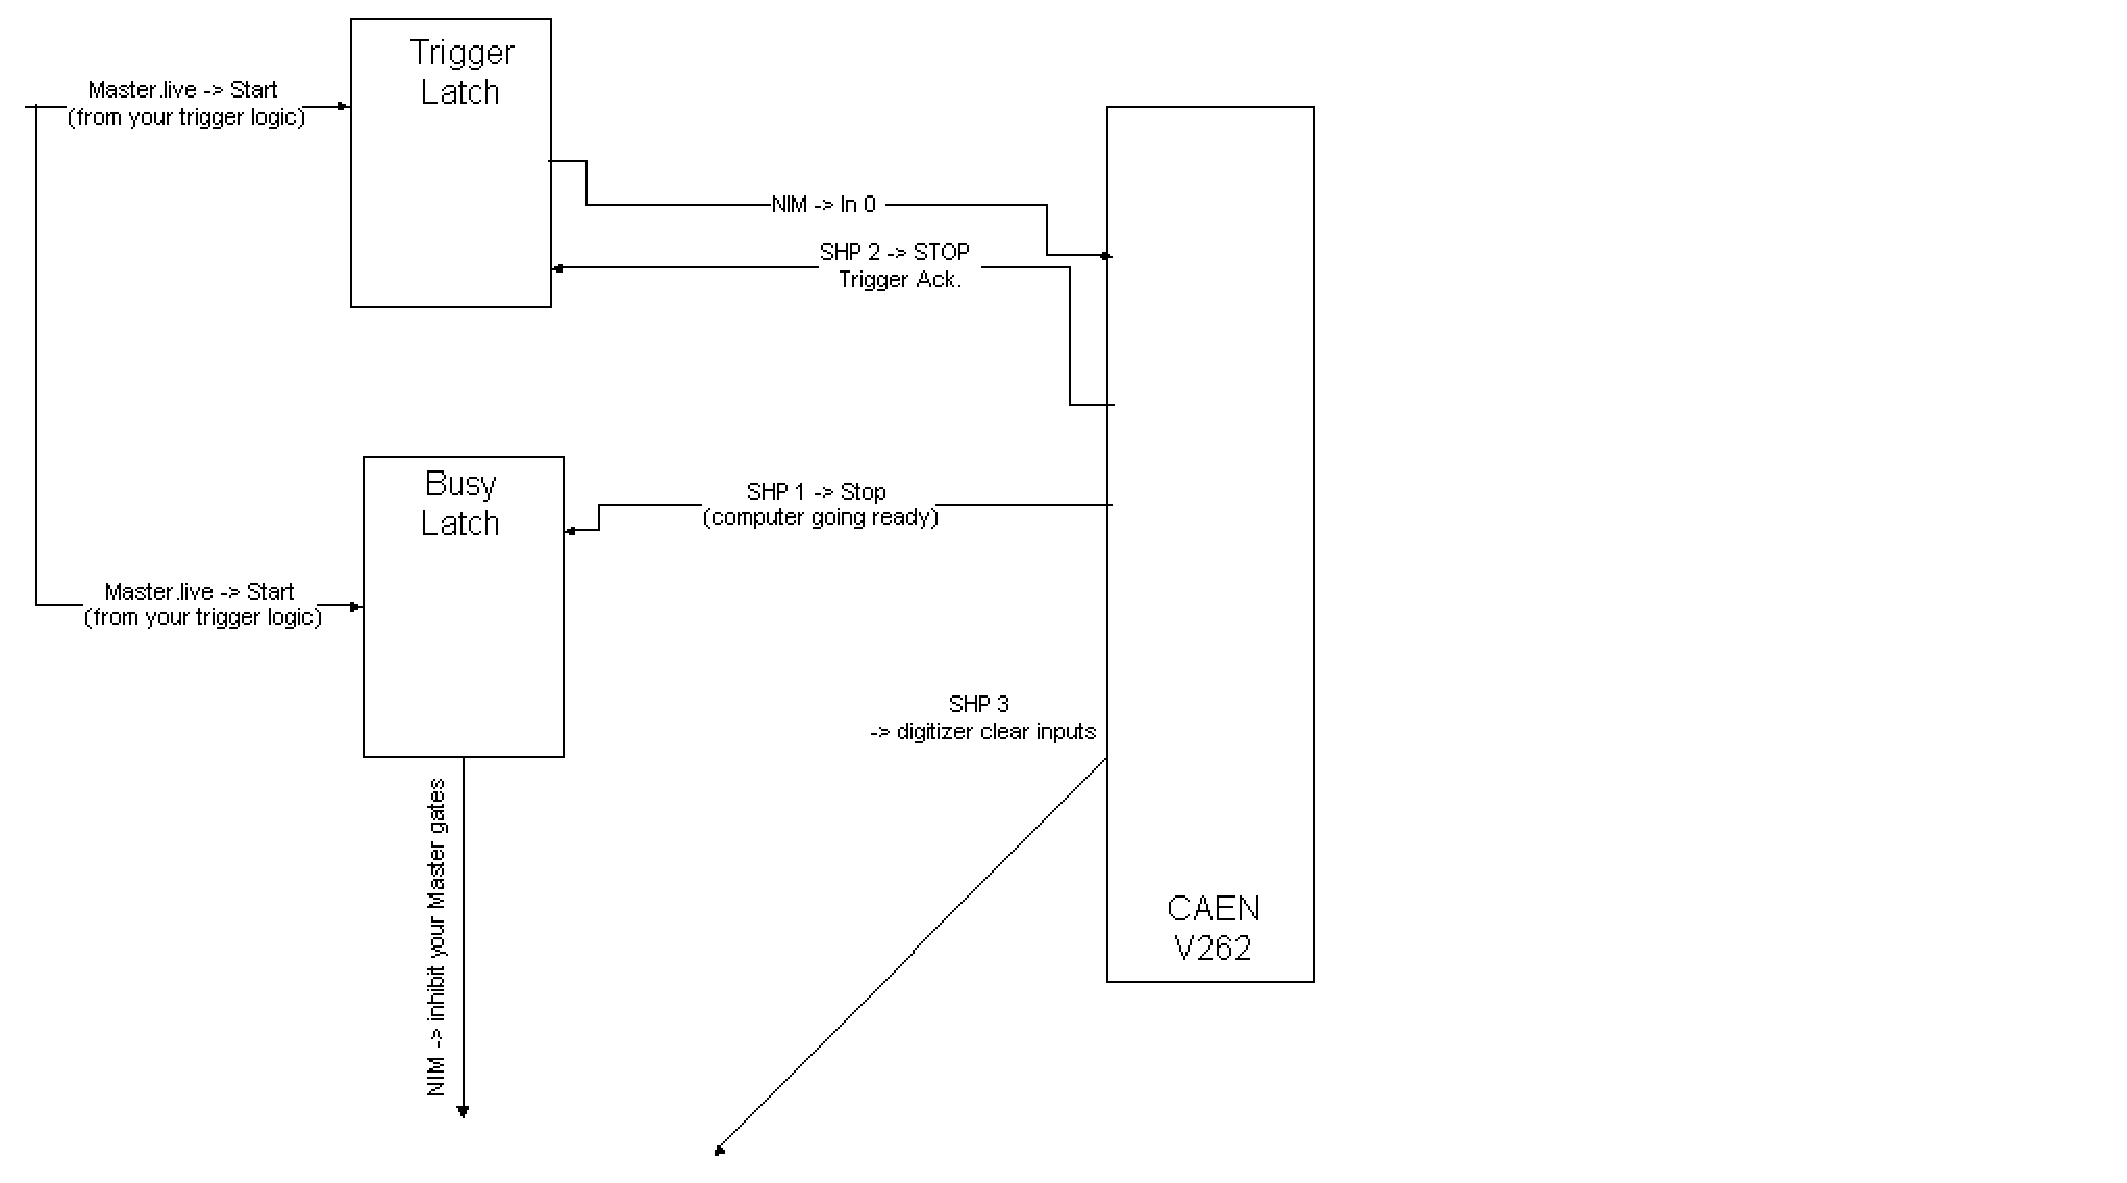
\includegraphics{VMETriggerelec.eps}}}{\htmlimage{VMETriggerelec.gif}}

	 \end{figure}
	
	The Master.live trigger comes in from your experiment trigger logic and, in the
	trigger latch produces a trigger that is held asserted as long as is required
	for the computer to react to it.  When the computer reacts to the trigger, it 
	pulses SHP 2 (Trigger acknowledge), de-asserting the computer trigger input.
	
	The Master.live trigger also sets the busy latch which inhibits further gates 
	from your experimental electronics. When the computer has finished reading an
	event it pulses SHP 3 (Module clears) which you can fan out and use to 
        clear digitization modules
	that have external clear inputs.  Finally, it pulses SHP 1 (Computer going
	ready) which clears the busy latch, enabling the electronics to gate the next
	event into the computer.
	
      \subsubs{CAMAC trigger requirements}{CAMACTrigger}
	    If you have selected a CAMAC trigger, you must use a single external latch 
	 to inhibit gates to the system while the computer is busy.  The computer
	 part of the trigger system consists of two modules:
	 \begin{description}
	    \item{CES CBD8210} The INT2 input of the VME CES CBD8210 CAMAC branch
	       highway driver is used as the computer trigger.	 The trigger CBD8210
	       must be set to branch 0.
	    \item{BiRa 3251}  The BiRa 3251 CAMAC NIM output register is used to
	       to provide several signals to the external electronics. This module
	       must be put in a specific CAMAC location: branch$=$0, Crate$=$2
	       Slot$=$19
	 \end{description}
	 If available, you may use channel 1 of an LRS2323A
	 CAMAC programmable gate generator in slot 21/22 instead of an external
	 latch.  If you do so, you need not externally stop this module.  If not used, these two
	 slots must be kept empty as the computer software will send function codes to
	 this slot as if the module were plugged in.  The remainder of this section assumes
	 that you are using an external (e.g. LRS 222 NIM GDG) latch rather than a CAMAC latch.
	 
	 The signal specifications are described in the table below:
	 \begin{table}[htb]
	 \caption{CAMAC trigger signal specifications}
	 \begin{tabular}{|l|r|}
	    \hline
	    {\bf Signal } 	& {\bf Meaning }		\\
	    \hline
	    CBD8210 INT2 	& Computer trigger.		\\
	    BiRa 3251 out1-8	& Module clears			\\
	    BiRa 3251 out 9	& Software busy begins		\\
	    BiRa 3251 out 10	& Going ready			\\
	    \hline
	 \end{tabular}
	 \end{table}
	 
	 Given this set of signal specifications, the suggested CAMAC	trigger logic is shown in the figure below.
	 \begin{figure}[htb]
	    \caption{CAMAC trigger electronics block diagram}
	    \texorhtml{\scalebox{0.5}{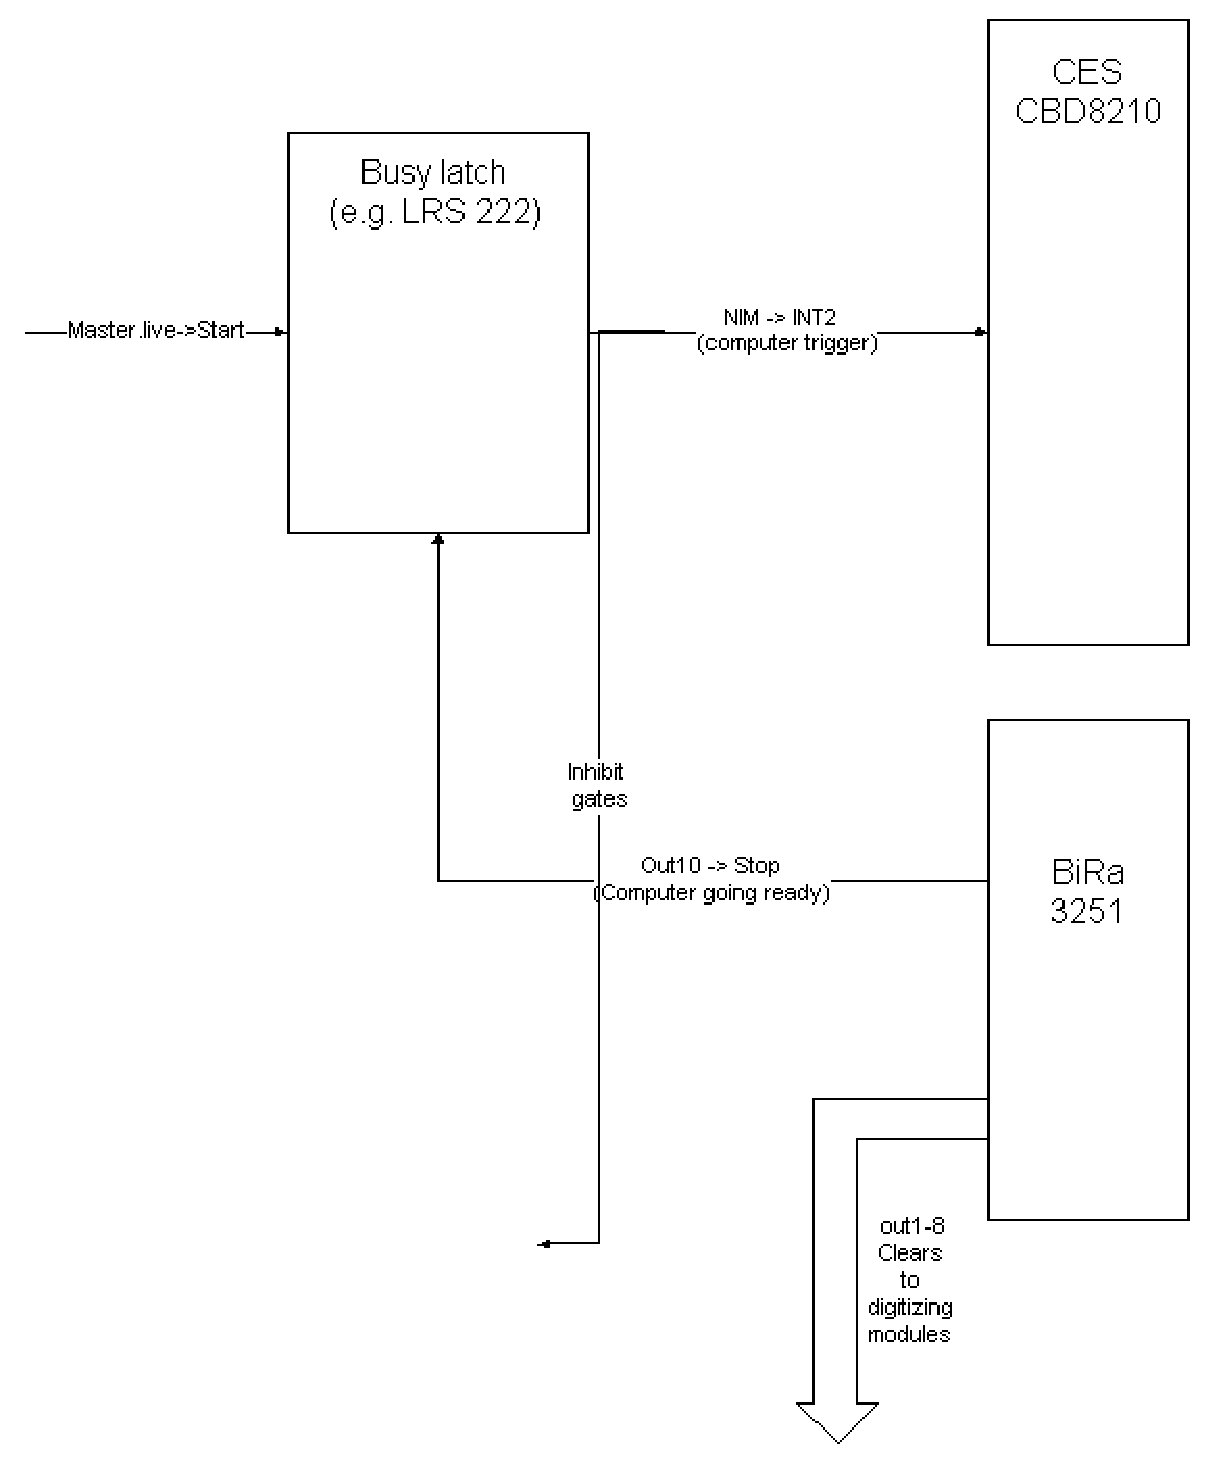
\includegraphics{CAMACTriggerelec.eps}}}{\htmlimage{CAMACTriggerelec.gif}}

	 \end{figure}
	 
	 It is not really necessary for the master gate to be latched by the the Busy latch,
	 before triggering the computer as the CES CBD8210 latches INT2 until reset by the
	 computer we suggest doing this, however becuase in this way, if you have an intermittent
	 cable, you won't hang the system; once a correct cable is plugged in, the trigger
	 will be sensed.
	 
	 The figure shows the busy latch set by the master.live.  The NIM output indicates 
	 that the trigger electronics should inhibit further gates.  
	 The NIMOUT Out 1-8 are pulsed after readout is complete and may be 
	 directly plugged in to digitizer 
	 clear inputs.  The NIMOUT Out 10 (Going ready) clears the NIM latch indicating that the computer
	 is ready for another gate.
	 
   \subs{Running your readout software}{Running}

   This section summarizes how to run the readout software you have created.  For 
   complete run time reference guide, see
   \link{Operating the readout software}[ (Section \ref{s:Operating})]{s:Operating}.
   This section only gives you enough information to get started with the readout software in
   a standalone manner.  Other documentation to be constructed will describe how to use the 
   run control software under the control of a graphical user interface front end associated with
   the staging system.

   A subset of the syntax of the command to start the readout program is:
   \begin{example}
   \computer{$<$Readout$>$} \human{Readout [{\dash\dash}window] [{\dash\dash}camac-trigger]}
   \end{example}
   where:
   \begin{description}
      \item{{\dash\dash}window} Indicates that you want to run the Readout with a full
	    tk (wish) interpreter installed.  The default is to run with tcl (tclsh)
	    only.  Use this if you want your readout program to have a graphical user
	    interface.
      \item{{\dash\dash}camac-trigger}   Selects the CAMAC trigger (see 
	 \link{Camac Trigger}[ (Section \ref{sss:CAMACTrigger})]{sss:CAMACTrigger}). The 
	    default is to use the VME trigger system (see
	    \link{VME Trigger}[ (Section \ref{sss:VMETrigger})]{sss:VMETrigger}).
   \end{description}
   
   After a copyright and author credit notice Readout will return the Tcl prompt:
   \begin{example}
   \computer{\%}
   \end{example}
   
   At this time you can type any Tcl command or Readout command extension.  If you have
   selected the {\dash\dash}window option, you may also type Tk commands.
   
   Readout maintains {\em run-variables} that can be modified via the tcl {\bf set} command.  These
   variables are write-protected when the run is active.  There are additional 
   {\em const-variables} that 
   may only be modified programmatically (the {\bf set} command will fail to modify them).  
   Run variables are intended for your use to document the experiment and run, while
   const-variables are intended to provide information about the program's internal
   status.
   
   The table below describes these variables:
   \begin{table}[htp]
      \caption{Variables maintained by Readout}
      \begin{tabular}{|l|l|l|}
      \hline
      {\bf Name}        & {\bf Contains}                        & {\bf Type} \\
      \hline
	 events		& Events accepted since last begin run  & const-variable \\
	 experiment	& Experiment description		& run-variable	\\
	 period		& Seconds beetween scaler readouts	& run-variable	\\
	 run		& Run number of current run		& run-variable	\\
	 starttime	& Time at which most recent run started	& const-variable \\
	 state		& State of the run Active | Paused | Inactive & const-variable \\
	 title		& Run title				& run-variable	\\
	 tkloaded	& true if {\dash\dash}window mode	& const-variable	\\
	 words		& Number of words of data taken since last begin & const-variable \\
      \hline
      \end{tabular}
   \end{table}
   
   The sample script below sets the run number, experiment description,
   scaler readout period and title for the next run.  
   This script will fail if the run is active:
   \begin{example}
   set run 123
   set experiment "Some radioactive beam experiment"
   set period 2     ;# Readout scalers every 2 seconds.
   set title \{Run with blank for beam background tests\}
   \end{example}
   Note that tcl accepts quoting either with `` and '' or with \{ and \}
   
   Readout extends the command set of tcl wih commands that allow you to control
   the readout run.  To get started you can use the commands (note all commands are
   case sensitive:
   
   \begin{table}[htb]
      \caption{Subset of run control commands}
      \begin{tabular}{|l|l|}
	 \hline
	 {\bf Command}		& {\bf Function } \\
	 \hline
	 begin			& Start a run.	\\
	 end			& End a run.	\\
	 exit			& Exit the program only if run is halted \\
      \end{tabular}
   \end{table}
      
   
\s{Operating the readout software}{Operating}
   This section describes in detail how to use the readout software.   Wherever
   possible, examples are provided so that you can see how the author expected
   features of the system to be used.  If you happen to come up with an application
   that you think is unique, interesting, and of general interest, please don't hesitate
   to contact us either via email at:
   \xlink{fox@nscl.msu.edu}{mailto:fox@nscl.msu.edu}
   or enter it as an enhancement request on our bug tracking system at:
   \xlink{http://bugzilla.nscl.msu.edu}{http://bugzilla.nscl.msu.edu}.
   
   \begin{iftex}
   The remainder of this section describes:
   \begin{itemize}
      \item Command options (Section \ref{ss:Options}).
      \item Added Tcl features (Section \ref{ss:TclFeatures}).
      \item The embedded TclServer (Section \ref{ss:TclServer}).
      
   \end{itemize}
   \end{iftex}
   \subs{Command options}{Options}
   
   The full form of the command to start your readout software is:
   \begin{verbatim}
   Readout --help
   Readout --version
   Readout [--camac-trigger] [--port=pnum] [--window]
   \end{verbatim}

   The first form of the command \verb+ Readout --help + prints out
   a summary of the command options:
   \begin{example}
   \human{Readout --help}
   \computer{
Readout 1.0

Purpose:
  Reads out experimental data to spectrodaq

Usage: Readout [OPTIONS]...
   -h      --help            Print help and exit
   -V      --version         Print version and exit
   -pINT   --port=INT        Enable tcl server functionality, next parameter is the port
   -w      --window          Use Tk interpreter if set (default=off)
   -c      --camac-trigger   Use  CAMAC triggers instead of VME (default=off)
   }
   \end{example}
   
   The second form of the command \verb+ Redout --version + prints out 
   the current version of the readout support framework.  Be sure to
   include this information in any problem reports you have For example::
   
   \begin{example}
   \human{Readout --version}
   \computer{Readout 1.0}
   \end{example}
   
   The final form of the command actually runs the readout program 
   in various modes and configurations.  The switches have the 
   following meaning:
   
   \begin{table}[htp]
      \caption{Command switches for Readout}
      \begin{tabular}{|l|l|l|}
	 \hline
	 {\bf Switch} & {\bf Parameter} & {\bf Meaning} \\
	 \hline
	 {\dash\dash}port   & Tcl Server port & Enables TclServer functionality on the 
					  selected port \\
	 {\dash\dash}window & N/A		& Enables Tk functionality \\
	 {\dash\dash}camac-trigger & N/A		& Enables CAMAC trigger. \\
	 \hline
      \end{tabular}
   \end{table}
   \subs{Added Tcl features}{TclFeatures}
      The readout program extends the Tcl/Tk language in several important ways:
      \begin{itemize}
	 \item Several commands are added to allow you to control
	    data acquisition
	 \item const variables have been added to allow Readout and
	    your application to display status information that cannot
	    be altered by the command interpreter.
	 \item Run Variables have been added to allow you to 
	    periodically log relevant time varying parameters to the
	    event stream.
	 \item State variables have been added to allow you to define
	    variables that are write protected during the run, and are
	    logged at state transitions to the event stream.
      \end{itemize}
      
      Added commands include:
      \begin{description}
	 \item{begin}  Enable data taking for a new run.  The  state variables
	    are write protected and internally maintained const variables are 
	    updated to reflect the current state of the system. Active runs
	    may be paused or ended.
	 \item{const} Defines or manipulates a const variable.  As far as Tcl/Tk is
	    concerned, a  const is a variable that refuses to be modified by 
	    scripts. It can, however be modified by the C/C++ application.  The
	    intention is that you use const variables to reflect internal program
	    state.
	 \item{end} Ends a run that is in progress.  Data taking is disabled and
	    the state variables are unprotected so that you can modify them
	    between runs.
	 \item{exit} Exit has been redefined to refuse to exit unless 
	    data taking is inactive (never begun or end was the last run
	    state command).
	 \item{pause} Pauses a run.  When the run is paused, state variables
	    are still locked, but data taking is disabled. Paused runs may be
	    resumed or ended.
	 \item{resume} Resumes a paused run.  Data taking is re-enabled.
	 \item{runvar} Creates or manipulates a run variable.  Run variables 
	    are automatically logged to the event stream with the same
	    periodicity as scaler reads.  This allows you to log parameters
	    that may change during the run simply by maintaning them in 
	    run variables.
	 \item{statevar} Creatse or manipulates state variables.  State
	    variables are write protected during runs (between begin and end).
	    The may be modified freely while the run is halted.  State
	    variables are logged to the event stream at the beginning of
	    the run.  State variable are intended to represent invariant
	    features of the run, for example, the run number, the beam, target
	    etc.
      \end{description}
      
      The readout software pre-defines several run variables and consts:
      
   \begin{table}[htp]
      \caption{Variables maintained by Readout}
      \begin{tabular}{|l|l|l|}
      \hline
      {\bf Name}        & {\bf Contains}                        & {\bf Type} \\
      \hline
	 events		& Events accepted since last begin run  & const \\
	 experiment	& Experiment description		& run variable	\\
	 period		& Seconds beetween scaler readouts	& run variable	\\
	 run		& Run number of current run		& run variable	\\
	 starttime	& Time at which most recent run started	& const         \\
	 state		& State of the run Active | Paused | Inactive & const \\
	 title		& Run title				& run variable	\\
	 tkloaded	& true if {\dash\dash}window mode	& const 	\\
	 words		& Number of words of data taken since last begin & const \\
      \hline
      \end{tabular}
   \end{table}
      
   \subsubs{begin}{begincommand}
   
   Begin starts a new run.  The format of the begin command is:
   \begin{example}
   begin
   \end{example}
   
   The following example starts a run and ends it after 20 seconds (must be
   run from Readout {\dash\dash}window):
   \begin{example}
   \computer{\% } \human{begin; after 20000 end}
   \end{example}
   The following example starts a run and ends it after at least 100,000
   events have been acquired.  It makes use of the events const (must be
   run from Readout {\dash\dash}window):
   \begin{example}
   \computer{\% }\human{ proc EndAfter \{nevents interval\} \{ 
			   global events 
			   if \{\$nevents <= \$events \} \{ 
			      end 
			   \} else \{ 
			      after \$interval \{EndAfter \$nevents \$interval \}
			   \} 
			   }
			   
   \computer{\% }\human{  begin; EndAfter 100000 10}
   
   \end{example}
   
   \subsubs{const}{constcommand}
	 The const command creates a tcl constant.  Tcl constants
      are named values that cannot be altered by tcl scripts.  Tcl
      constants can, however, be modified from the C/C++ application.
      You can use const values as constants in your Tcl scripts,
      or alternatively to reflect status values maintained by the
      C/C++ software.   The format of  the const command is:
      \begin{example}
      \computer{\% }\human{const {\it name ?value?}}
      \end{example}
      
      Where:
      \begin{description}
	 \item{name} is the name of the constant.
	 \item{value} is an optional value for the constant.
	    if omitted, the const will have the value 0.
      \end{description}

      Normally consts will be created from the C++ code.
      See
      \link{const ``variables''}[
      (Section \ref{sss:constvariables})]{sss:constvariables} for
      more information about accessing const's from user code.
      
   \subsubs{end}{endcommand}
      The end command ends the currently active run:
      \begin{example}
	 \computer{\% }\human{end}
      \end{example}
   \subsubs{exit}{exitcommand}
      The exit command exits the readout program.  This is a replacement
      for the standard Tcl {\em exit} command.  If there is an 
      active or paused run, exit indicates this and refuses to exit:
      \begin{example}
	 \computer{\% }\human{begin}
	 \computer{\% }\human{exit}
	 \computer{A run is active and must be halted before exiting}
	 \computer{\% }\human{end}
	 \computer{\% }\human{exit}
	 \computer{$< >$}
      \end{example}
   \subsubs{pause}{pausecommand}
      The pause command pauses an active run.  If the run
      is not active an error message is emitted.  Once paused,
      a run can either be resumed or ended.
      \begin{example}
	 \computer{\% }\human{pause}
      \end{example}
   \subsubs{resume}{resumecommand}
      The resume command resumes an active run.  If the run
      is not puased an error message is emitted.  Once active,
      a run can either be paused or ended.
      \begin{example}
	 \computer{\% }\human{resume}
      \end{example}
   \subsubs{runvar}{runvarcommand}
      Manipulates the run variables.  A run variable is an item that is
      periodically logged to the event stream.  It is allowed to vary 
      during the run.  The runvar command can be used to:
      \begin{itemize}
	 \item Create a new runvariable and optionally assign it a
	    value:
	    \begin{example}
	       \computer{\% }\human{runvar newvar ?value?}
	    \end{example}
	    creates a new run variable named {\em newvar} if
	    {\em value} is supplied the new variable's initial
	    value is set to {\em value}.
	 \item List the set of run variables that are defined:
	    \begin{example}
	       \computer{\% }\human{runvar -list ?glob-pattern?}
	    \end{example}
	 \item Delete a run variable:
	    \begin{example}
	       \computer{\% }\human{runvar -delete varname}
	    \end{example}
      \end{itemize}
   \subsubs{statevar}{statevarcommand}
      The {\em statevar} command manipulates state variables.  
      State variables are varialbes that are write protected
      while a run is active.   They are intended to contain 
      information that documents the conditions of a run.
      For example, a statevar named {\em beam} might have
      the specifications of the beam during the run. 
         State variables are logged to the event stream when
      the run becomes active. The statevar command allows you to:
      \begin{itemize}
	 \item Create a new state variable.
	    \begin{example}
	       \computer{\% }\human{statevar name}
	    \end{example}
	    Creates a new state variable: {\em name}.
	 \item List the set of state variables defined whose names
	    match a glob pattern.
	    \begin{example}
	       \computer{\% }\human{statevar -list ?glob-pattern?}
	    \end{example}
	    Lists the set of state variables whose names match
	    the pattern {\em glob-pattern}.  Note that if this 
	    optional parameter is not supplied, all statevars will
	    be listed.
	 \item Delete a state variable.
	    \begin{example}
	       \computer{\% }\human{statevar -delete varname}
	    \end{example}
      \end{itemize}

   \subs{The embedded TclServer}{TclServer}
      The readout software has embedded TclServer functionality.
      This means that it is possible for remote software to establish
      connections to the Readout software and issue arbitrary
      Tcl commands executed by Readout.  This functionality allows one to:
      \begin{itemize}
	 \item Write control panels that can run on systems remote to the
	    Reaout program.
	 \item Remotely update the values of state and run variables.
	 \item Remotely inquire about the state of the system or the
	    value of any of the variables (normal, const, state or run) 
	    defined by the software.
      \end{itemize}
      
      TclServer is enabled by using the --port switch on the command line
      that starts up the Readout. See 
      \link{Operating the readout software}[
       (Section \ref{s:Operating})]{s:Operating} for the format of this switch.
       
       Since remote software can perform arbitrary operations via the
       TclServer security is an issue.  The TclServer initially 
       comes up only accepting connections from the local system.
       The TclServer registers the {\em serverauth} command to 
       control host based access to the TclServer.
       
       The serverauth command can be used to:
       \begin{itemize}
	  \item Enable access to the TclServer for a host based on 
	     its name or IP address:
	     \begin{example}
		\computer{\% }\human{serverauth add hostorip}
	     \end{example}
	 \item Disallow access to a previously allowed host:
	    \begin{example}
	       \computer{\% }\human{serverauth remove hostorip}
	    \end{example}
	 \item Show the list of hosts that are authorized to connect
	    to the TclServer:
	    \begin{example}
	       \computer{\% }\human{serverauth list}
	    \end{example}
	    Note that the list will be a set of doublets.  Each doublet
	    has the hostname and the correspond the IP address.
       \end{itemize}
       
\s{Structure of the Program}{Readoutstructure}
   This section describes the structure of the readout program. It is 
   intended as background material for people who are making 
   significant modifications to the Readout software.  For an
   internals reference, see 
   \link{Reference documentation for the internals of Readout}[
       (Section \ref{s:Readoutdoxygen})]{s:Readoutdoxygen}.
       
   This section describes:
   \begin{iftex}
   \begin{itemize}
      \item The thread structure of the program and how to syncrhonize.
      \item Major classes and objects you will have to interact with.
      \item Initialization flow of control.
      \item State transition flow of control.
      \item Event handling flow of control.
   \end{itemize}
   \end{iftex}
   \subs{How the system is threaded}{Threading}
      The readout software is a highly threaded system.  Threading is used
      to allow the software to cleanly expect and respond to several 
      types of external stimulii.  
      
      The threading is done on top of the
      NSCL DAQ programming framework.   % BUGBUGBUG \xlink
      The program framework supports separate threads for each stimulus
      a program may wait for.  The threads autonomously wait for a simulus
      and, when one is recieved, acquire a single global synchronization
      mutex.  This has the effect of simulating an open ended event 
      based programming system within the context of multithreading.
      
      In addition to a standard set of event types, the program framework
      supports the concept of guest event processing frameworks.  Tcl or
      Tk run as a guest event processing framework. In handling the Tcl 
      interpreter, the assumption is that most Tcl commands (e.g. set) 
      dont' require synchronization.  Extensions to the base interpreter
      are derived from a CDAQTCLProcessor which acquires the syncronization
      mutex prior to transferring control to the object's operator().
      
      If scripts require synchronization, the Tcl interpreters also support
      the {\em sync} command.   The sync command takes a single argument,
      which is a script that is executed with the global mutex held.
      
      The global mutex is a counting mutex, so there's no penalty to 
      acquire it several times within a single thread, however you must
      release the mutex the same number of times it has been acquired.
      
      The code example below shows how to use the global syncronization
      mutex in your code if you work outside the limits of the program
      framework:
      
      \begin{example}
      #include <SpectroFramework.h>
      ...
      
      // Unsynchronized.
      
      CApplicationSerializer::getInstance()->Lock() 
      
      // this code is synchronized.
      
      CApplicationSerializer::getInstance()->UnLock();
      
      // Unsyncrhonized
      \end{example}
      
      The figure below shows the start/stop relationships between the 
      threads of the system:
      
      	 \begin{figure}[htb]
	    \caption{Thread Relationships}
	    \texorhtml{\scalebox{0.5}
			      {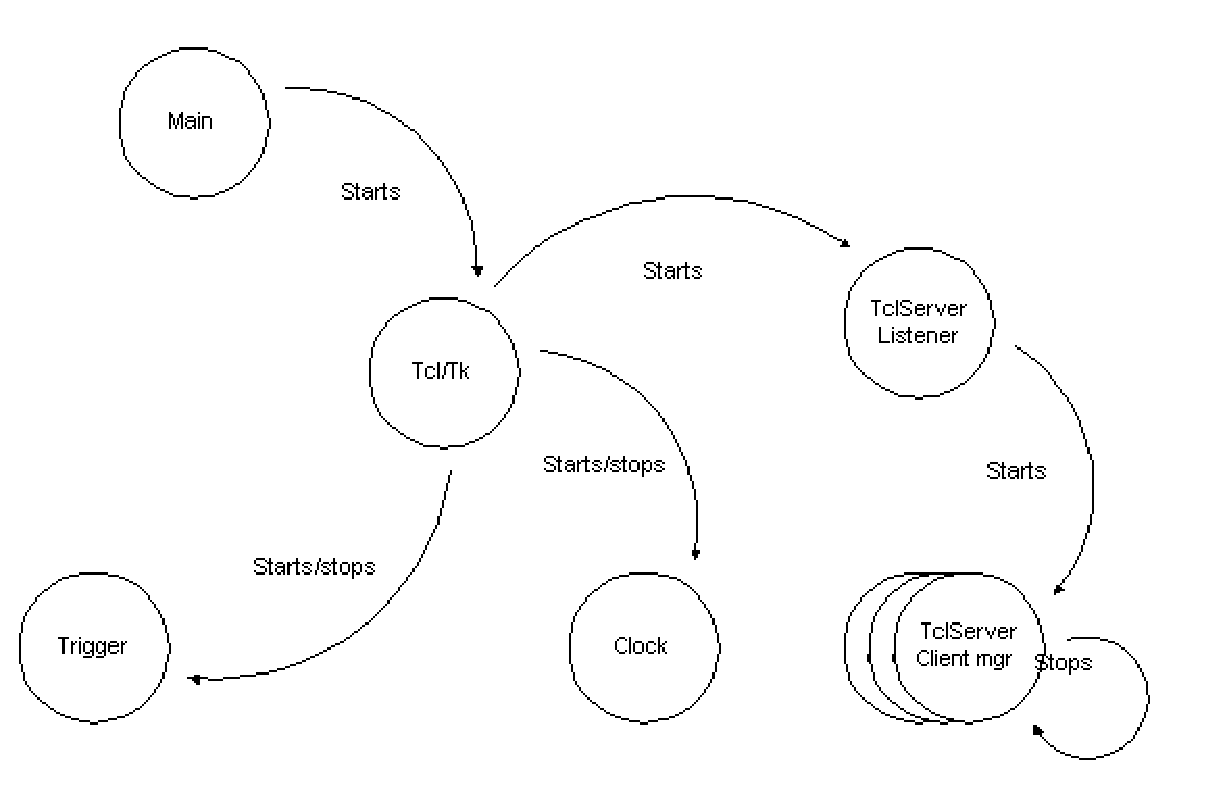
\includegraphics{Threadingdiagram.eps}}
			      }{\htmlimage{Threadingdiagram.gif}}

	 \end{figure}

      \begin{itemize}
	 \item The main thread starts off the Tcl interpreter and
	    enters a sleep loop periodically checking a flag that
	    is set when the application should exit.  When the application
	    should exit, the main process executes the exit(2) system 
	    service, which ends all threads.
	 \item The Tcl interpreter thread, on startup determines if TclServer
	    functionality has been requested.  If so, the serverauth command
	    is registered and a CTCLListener object is creaeted and run
	    in its own thread.
	 \item The CTCLListener thread listens for connections on the
	    specified Tcp/Ip port.  When a connection is honored, a 
	    CTCLServer object is started and run in its own thread. 
	    The CTCLServer object accepts commands from the client
	    and executes them until the client exits.  All client scripts
	    are serialized with respect to each other and also run with
	    the global serialization mutex enabled, however, they will
	    not be synchronized with respect to scripts and commands 
	    executed in the main Tcl/Tk thread, unless those scripts and
	    commands are run within the {\em sync} command.
	 \item The Tcl/Tk thread, in response to a begin command e.g. will
	 start off two threads.  The Trigger thread watches for event triggers
	 and, in response to them, reads out events from the hardware.
	 The Clock thread keeps track of elapsed run time and triggers scaler
	 readouts.  The Tcl/Tk also kills these threads in response to commands
	 ({\em end}, {\em pause}) that deactivate the run.  Since these 
	 commands run synchronized with respect to both the trigger and clock
	 thread, there's no danger the trigger thread or clock thread are
	 asked to terminate in mid event.
      \end{itemize}
      
   \subs{Major classes and objects}{Classes}
      Several majore classes and objects (instances) of those classes are
      described in this section.  Knowing your way around these classes
      helps you both to understand the way the readout program works
      as well as how to extend it.  This section will also describe:

      \begin{itemize}
	 \item How to locate the key objects.
	 \item Major member functions for each of the classes.
       \end{itemize}
       
       For detailed reference information on the software, see
       the Doxygen documentation of they software referenced
       in \link{Reference documentation for the internals of Readout}[
	  (Section \ref{s:Readoutdoxygen})]{s:Readoutdoxygen}.
	  
      The figure below shows the major classes and their relationships:

      \begin{figure}[htb]
	 \caption{Major class relationships}
	 \texorhtml{\scalebox{0.5}
			   {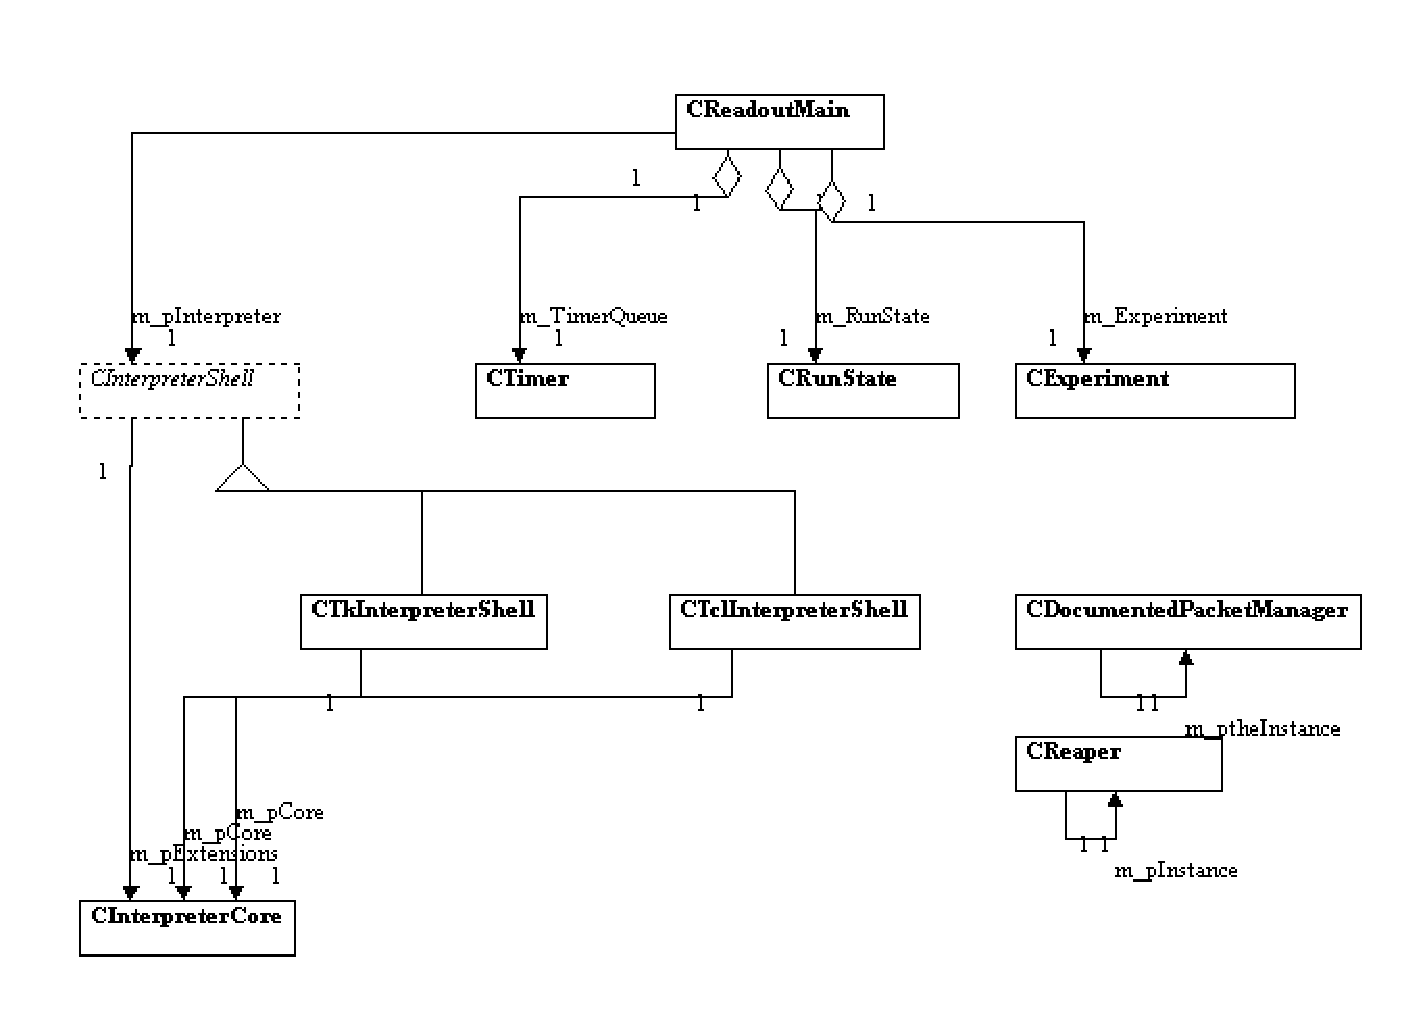
\includegraphics{MajorClasses.eps}}
			      }{\htmlimage{MajorClasses.gif}}

	 \end{figure}   
      
      \begin{description}
	 \item{CReadoutMain} is a singleton object. Its operator()
	    gets initial control.  Note that usually, you will override
	    this class to tailor its virtual functions (see 
	    \link{Modifiying the Readout skeleton}[
	       (Section \ref{ss:Modifying})]{ss:Modifying}).
	       CReadoutMain's member functions allow you to get 
	       pointers to the instances of the classes it contains:
	       
	       \begin{description}
		  \item{CTimer\& \function{getClock()}}
		     Returns a reference to the clock manager.  The
		     clock manager runs when the run is active and
		     is a scheduler of timed events.
		  \item{CRunState* getRunState()}
		     Returns a pointer to the run state object.  The run state
		     object encapsulates the state machine that
		     describes the current state of the run and
		     allowed state transitions.  See:
		     \link{System State Machine}[
			(Section \ref{ss:StateMachine})]{ss:StateMachine}.
		  \item{CExperiment* getExperiment()}
		     Returns a pointer to the experiment.  The experiment
		     object houses all of the functionality of the experiment itself,
		     divorced from the flow control, command processing and so 
		     forth.
		  \item{CInterpreterShell* getInterpreter()}
		     Returns a pointer to the Interpreter shell object.  This will 
		     actually be either a CTkInterpreterShell or a CTclInterpreterShell.
		     Each of these classes doubly inherits from CInterpreterShell and
		     from CInterpreterStartup.  CInterpreterStartup gives Interpreter
		     shells the behavior of a guest event loop running Tcl or Tk.
		     While CInterpreterShell gives the property of holding a core set
		     of common interpreter extensions regardless of whether or not
		     the underlying interpreter is a Tcl or Tk interpreter.
	       \end{description}
	       \htmlrule
	 \item{CTimer} is a class that manages timed events.  The
	    CReadoutMain class/objects maintains one of these for use by
	    the experiment.  When the run is active, this timer is ``turned on'',
	    and starts scheduling events.  Normally the experiment will register
	    a scaler trigger that will fire periodically to read out run time
	    scalers.  Major function of CTimer are:
	    
	    \begin{description}
	       \item{void \function{Start}(int \param{ms}, bool \param{reset=false})}
		  Enables the timer
		  to schedule events.  {\param ms} is the timer resolution in 
		  milliseconds.  The timer will wake up every {\param ms} and
		  check for events that have come due. {\param reset} 
		  should be set true if you want the object's concept of elapsed
		  time to be reset to zero.
	       \item{void \function{Stop}()} Disables the timer.  The timer
		   will no longer schedule events.
	       \item{int \function{GetElapsedTime}()} Returns the elapsed
		  time in milliseconds.  
	       \item{void \function{EstablishEvent}(CTimedEvent\& \param{rEvent}}
		  Adds the object \param{rEvent} to the list of items that
		  the timer will periodically schedule.
	    \end{description}
	    \htmlrule
	 \item{CRunState} Run state objects encapsulate the state machine
	    that defines legal transitions between states of the run and the
	    current state as well.  Major functions are:
	    
	       \begin{description}
		  \item{CRunState::RunState \function{getState}()}
		     Returns the current state.  The CRunState::RunState
		     data type is an enumerated data type with values:
		     \param{Inactive}, \param{Active}, or \param{Paused}.
		  \item{bool \function{Allowed}(CRunState::RunState \param{NewState}}
		     Returns \param{true} if it is now legal to make a transition
		     to the state \param{NewState}, false if not.  note as
		     well that the state transition functions described below
		     also throw a CBadTransition exception if the transition is
		     not legal.
		  \item{void \function{Begin}()} Transition to the Active state.
		  \item{void \function{End}()} Transition to the Inactive state.
		  \item{void \function{Pause}()} Transition from Active to
		     Paused.
		  \item{void \function{Resume}()} Transition from Paused to
		     Active.
		  \item{string \function{getStateName}()} Returns a string
		     version of the name of the state.
	       \end{description}
	       \htmlrule
	  \item{CExperiment} is a class that contains configuration 
	     information and functions relelvant to the experiment itself. Major
	     member functions include:

	    \begin{description}
		\item{void \function{AddEventSegment}(CEventSegment* \param{pSegment})}
		   Adds an event segment to the readout.  For more about 
		   event segments, see:
		   \link{How to structure your readout}[
		    (Section \ref{sss:newreadout})]{sss:newreadout}.
		\item{void \function{RemoveEventSegment}(CEventSegment* \param{pSegment})}
		   Removes an event segment from the readout. 
		   For more about 
		   event segments, see:
		   \link{How to structure your readout}[
		    (Section \ref{sss:newreadout})]{sss:newreadout}.
		\item{void \function{EstablishTrigger}(CTrigger* \param{pTrigger})}
		   Replaces the current trigger object with a new one. Trigger modules
		   supply a mechanism to watch for the event readout trigger.  For more
		   about the CTrigger class, see:
		   \link{Specifying a trigger}[
		      (Section \ref{ss:TriggerSpec}]{ss:TriggerSpec}.
		\item{void \function{EstablishBusy}(CBusy* \param{pBusy})}
		   Replaces the current Busy management object with a new one.
		   The CBusy object provides a mechanism to manage the 
		   computer busy signal required by experimental electronics.
		   For more about the CBusy class, see:
		   \link{Specifying a busy manager}[
		      (Section \ref{ss:BusySpec})]{ss:BusySpec}.
		\item{void \function{AddScalerModule}(CScaler* \param{pScaler})}
		   Adds a scaler module to the list of modules that will be read
		   on a scaler trigger.  Note that CScalerBank is derived from
		   CScaler so you can hierarchically organize the readout.
		\item{void \function{RemoveScalerModule}(CScaler* \param{pScaler})}
		   Removes an existing scaler module from the scaler readout.
	     \end{description}
	     \htmlrule
	    \item{CInterpreterShell} encapsulates the Tcl or Tk interpreter
	       relevant to the readout system. Complete coverage of the
	       Tcl/Tk interpreter structure will be given in several sections
	       of \link{Tailoring the software}[
		  (Section \ref{s:Readouttailoring})]{s:Readouttailoring}.
	       The main functions you will need is 
	       CInterpreterCore* \function{getInterpreterCore}() 
	       which gets the interpreter core.  The interpreter core object
	       is the set of extensions that Readout has layered on to
	       the base Tcl/or Tk interpreter, and CTCLInterpreter\&
	       \function{Interp}() which gets the interpreter object
	       itself.
	       \htmlrule
	    \item{CReaper} monitors threads that must be deleted on exit.
	       Threads are normally objects of type derived from CEvent.
	       Deleting dynamically created CEvent objects is problematic as
	       it must be done by some `force' outside the thread itself.
	       CReaper is a singleton class that can be used to ensure that
	       dynamically created thread objects are deleted on exit.  Key 
	       member functions are:
	       \begin{description}
		  \item{CReaper* \function{getInstance}()}
		     Returns a pointer to the single reaper object.
		  \item{void \function{Add}(CEvent* \param{pEvent})}
		     Called by a thread on entry to add itself to the reapers
		     list of monitored processes.
	       \end{description}
	       A typical sequence of code might be:
	       \begin{example}
		  CReaper::getInstance()->Add(this);   // Auto delete on exit.
	       \end{example}
      \end{description}
   \subs{Initialization flow control}{Initialization}
      To understand where to add code to modify the behavior
      of Readout you must understand how Readout initializes.
      The figure below is a flowchart of this initialization process.
      \begin{figure}[htb]
	 \caption{Initialization flow chart}
	 \hyperimage{InitializationFlow}
      \end{figure}
      
      After command line switches are parsed and decoded, Experiment 
      initialization takes place.  This involves creating a CExperiment
      object and initializing its elements.  All initialization of CExperiment
      are done in the context of the main thread.
      
      Normally, CReadoutMain is subclassed, and you override two member
      functions to initialize the CExperiment object for your application.
      
      These functions are:
      
      \begin{description}
	 \item{void \function{SetupReadout}(CExperiment\& \param{rExperiment})}
	    \function{SetupReadout} invokes 
	    CExperiment::\function{AddEventSegment} to register segments
	    of the application's readout with the experiment.  When an event
	    trigger is received, the trigger thread will iterate through the event
	    segments, reading each out in the order it was registered.
	 \item{void \function{SetupScalers}(CExperiment\& \param{rexperiment})}
	 \function{SetupScalers} invokes CExperiment::\function{AddScalerModule}
	 to setup the desired scaler readout.  When a scaler trigger is
	 recieved, the Timer thread will iterate through the scaler modules
	 that have been added and read each out in registration order.
      \end{description}
      
      Interpreter setup is slightly more complex because the interpreter runs
      in a separate thread.  The Readout initialization software first
      checks for the presence of the {\dash\dash}window switch.  If present,
      a Tk interpreter is started off, if not, a Tcl interpreter.  
      
      Regardless of the interpreter started, it retains a object of 
      CInterpreterCore.  That object is responsible for registering all
      extensions to the command interpreter.  After registering the standard
      extensions, in order it invokes three CReadoutMain member functions
      to allow the user to add any interpreter extensions requried by the
      application.  These member functions are called in the context of the
      Interpreter thread.  The CReadoutMain functinos called are virtual 
      functions that can be overridden by the user to supply extensions
      without modifying the source of the framework.
      
      
      The functions called are:
      \begin{description}
	 \item{void \function{AddUserCommands}(CExperiment\&           \param{rExperiment},
								     CInterpreterStartup\& \param{rStartup},
								     CInterpreterCore\&     \param{rCore})}
	    \function{AddUserCommands} is expected to create and register
	    any application specific commands that further extend the interpreter.
	    Note that CInterpreterStartup::\function{Interp}() allows you to
	    retrieve the interpreter object.
	 \item{void \function{SetupStateVariables}(CExperiment\&       \param{rExperiment},
								     CInterpreterStartup\& \param{rStartup},
								     CInterpreterCore\&     \param{rCore})}
	   \function{SetupStateVariables} is expected to add any state
	   variables your application wants to monitor.
	 \item{void \function{SetupRunVariables}( CExperiment\&           \param{rExperiment},
								     CInterpreterStartup\& \param{rStartup},
								     CInterpreterCore\&     \param{rCore})}
	    \function{SetupRunVariables} is expected to add any run
	    variables your application wants to maintain.
      \end{description}
      
      
      Once all extensions have been initialized, if the {\dash\dash}port 
      switch specified a TclServer port, Readout will initiate a thread
      to listen for TclServer client connections.  This sequence of operations
      ensures that by the time the first TclServer connections are honored
      and the Tcl/Tk interpreter prompt is issued to stdin, all standard and
      application specific extensions have been initialized and installed in 
      the interpreter.
      
      
   \subs{State transition flow control}{StateMachine}
   
   The readout software manages data acquisition as a simple state machine. 
   The state machine is described in the figure 
   \link{labelled Readout State Machine}[
      (Figure \ref{f:statemachine})]{f:statemachine}.
   
        \begin{figure}[htb]
	 \caption{Readout State Machine}\label{f:statemachine}
	 \hyperimage{RunStateDiagram}
      \end{figure}
  
   Descriptively:
   \begin{description}
      \item{Inactive}  In this state, no data is being taken.  The 
		   trigger thread is not alive.  When the program starts,
		   data acquisition is in the inactive state.  Valid transitions
		   occur on the \command{begin}  command (which requests
		   a transition to the Active state), and the \command{end}
		   state (which requests that the program exit).
      \item{Active} In this state data is being acquired.  There is a trigger
	 thread that is actively responding to event triggers by reading out
	 associated events.  The allowed transitions are initiated by the
	 commands: \command{end} (which requests a transition to the
	 inactive state), and \command{pause} (which requests a 
	 transition to the paused state).
      \item{Paused}  In this state, the run is suspended for possible 
	 resumption.  Valid state transitions are initiated by the commands:
	 \command{resume}, (which requests that the run be returned to
	 the active state so that data taking can be continued) and 
	 \command{end} (which requests that the run be exited).
   \end{description}
   
   All state transitions are initiated from outside the trigger thread. For
   example, command execution will happen either in the Tcl/Tk guest
   event loop thread, or within one of the TclServer threads.
   The flow control breaks into two types of transitions.  Those that initiate
   event taking (transitions into the active state), and those that 
   end event taking (transitions into the inactive, or paused state).
   
   Transitions into the Active state will call the CExperiment::Start().
   This function will setup and start two threads of control.  The clock 
   thread will manage the timing of scaler readouts and keep a run
   elapsed time for elapsed time fields of the buffer.  The trigger thread
   wil monitor triggers and, on receipt of one, Call CExperiment::ReadEvent()
   in the context of its thread to read the event.
   
   Transitions out of the Active state will call the CExperiment::Stop()
   member function.  The trigger thread is halted by calling it's stop function.
   The stop function sets a stop flag in the threads member data and does
   a Join operation to wait for the thread to actually exit.  The clock thread
   is also halted in the same way.  Without an active trigger thread to 
   initiate event readout and a clock thread to initiate periodic scaler readout,
   the run is effectively halted.
   
   \subs{Event handling flow of control}{EventHandling}
   Events are read out in response to a trigger.  The trigger
   is represented as a function object derived from CTrigger.
   The object's \function{operator()} returns a true value when
   a trigger has been received.
   
   Triggers are polled for in a separate trigger thread.  This design
   allows the system to be responsive to commands while keeping
   the average trigger latency very low (measured at about 3$\mu$sec).
   The trigger thread polls for the trigger in an inner loop while an outer 
   loop checks periodically to see if it has been asked to exit.
   
   The trigger loop thread object contains a pointer to the experiment
   object. The main trigger loop is shown below:
  
  \begin{example}
  while(!m_Exiting) \{
    struct timeval mutexstart;
    struct timeval mutexend;
    struct timezone tz;		// Unused but required for gettimeofday(2).
    int dwell;
    //
    // Lock the mutex and process triggers for the 
    // dwell time. The trigger is checked several times 
    // to amortize gettimeofday().
    //
    gettimeofday(&mutexstart, &tz);
    CApplicationSerializer::getInstance()->Lock();
    do \{
      for(int i = 0; i < 500; i++) \{
        int triggers=0;
        if((*m_pTrigger)()) \{	// Read an event...
            m_pExperiment->ReadEvent();
            if((triggers++) >= m_nTriggerdwell) 
		break; // Check elapsed time.
	\}
      \}
      // If we've held the mutex for longer than m_msHoldTime,
      // release the mutex so that other threads get a chance to run.
      //
      gettimeofday(&mutexend, &tz);
      int secdif = mutexend.tv_sec - mutexstart.tv_sec;
      mutexend.tv_usec += SECOND*secdif;
      dwell = (mutexend.tv_usec - mutexstart.tv_usec)/MILISECOND;
    \} while(dwell < m_msHoldTime);
    CApplicationSerializer::getInstance()->UnLock();
  \}
   \end{example}
   
   
      Several points to note:
      \begin{itemize}
	 \item The trigger thread does not re-acquire the serialization
	    mutex for each trigger check.  Instead it holds it for a time
	    no less than m\_msHoldTime milliseconds, and not much longer
	    than that (at most 500 trigger poll times longer than that).
	    This amortizes mutex acquisition, and system calls to 
	    determine how long the mutex has been held over several trigger
	    checks and perhaps several event readouts.
	 \item Each time the mutex iss released, the thread checks
	    its exit flag (m\_Exiting) to determine if it is time to exit.
	 \item Since event readout can be long compared to trigger
	    checks, at most m\_nTriggerdwell triggers are accepted
	    before checking to see if it is time to release the mutex.
      \end{itemize}

   Event readout, once initiated executes within the context of the 
   trigger thread with the global synchronization mutex already acquired.
   
\s{Tailoring the software}{Readouttailoring}

   This section describes how to some more advanced tailoring of
   the readout software.   
   
   \begin{iftex}            % html mode gives a list of subsecs.
   Subsections describe:
      \begin{itemize}
	 \item How to create user specific trigger objects
	    (see Section \ref{ss:TriggerSpec}).
	 \item How to specify a user specific computer busy
	     object (see Section \ref{ss:BusySpec}).
	 \item How to define event packets that are documented
	     in the begin run documentation buffers
	       (see Section \ref{ss:Packetdocs}).
	 \item How to add application specific commands to to
	    the program (see Section \ref{ss:ReadoutExtendCommands}
	 \item How to add application specicif variables, and
	    access them from within the application.
      \end{itemize}
   \end{iftex}

   \subs{Specifying a trigger manager}{TriggerSpec}
      The trigger manager is responsible for determining
      when an event is ready to be read out.
      Specifying an alternate trigger is a matter of:
      \begin{itemize}
	 \item Coding a new trigger object.
	 \item Creating an instance of this trigger
	 \item Ensuring that the custom trigger is
	    registered with the experiment object.
      \end{itemize}
   
      The functionality of checking a trigger is encapsulated in
      objects that are derived from the class CTrigger.
      Concrete classes derived from CTrigger must implement the
      function:
      \begin{example}
	 virtual bool \function{operator()}();
      \end{example}
      This function is called to poll the trigger hardware
      and is expected to return {\em true} if a pending trigger
      is ready.
   
      The following sample code shows a Test trigger class
      that claims the system always has a trigger to process:
      \begin{example}
        #include <CTrigger.h>
        class CTestTrigger : public CTrigger
	\{
	  public:
	    virtual bool operator()() \{
	       return true;
	    \}
	\};
      \end{example}
      
      Once coded, the new trigger object must be instantiated
      and installed in the experiment.  This should be done in 
      the users's SetupReadout function.  The code fragment
      below shows how this is done:

   \begin{example}
      void
      MyReadout::SetupReadout(CExperiment\& rExperiment)
      \{
	 CReadoutMain::SetupReadout(rExperiment);
	 rExperiment.EstablishTrigger(new CTestTrigger);
	 
	 \ldots
	 
      \end{example}
        

   
   \subs{Specifying a busy manager}{BusySpec}
      Busy managers are responsible for indicating when the
      computer is {\em dead} or unable to accept a new trigger.  
      The computer is dead in the time between a trigger
      occuring and the event readout completing.  It is also
      dead when the run is paused or halted.
      
      Substituting a user written busy manager for one of the
      standard busy managers is a matter of:
      \begin{itemize}
	 \item Writing a class derived from CStatusModule
	 \item Creating an instance (object) of that class
	 \item Registering that object as the Busy module
	    used by the experiment.
      \end{itemize}
      
      To write a busy manager, subclass the CStatusModule 
      class.  The important functions that must be defined are:
      \begin{description}
	 \item{void \function{GoBusy}()}  Called when the
	    system must assert the busy for software reasons
	    (e.g. end of run).
	 \item{void \function{GoClear}()} Called when the
	    system should deasser the busy.  This is called
	    at the end of each event and at the beginning of
	    each run, for example.
	 \item{void \function{ModuleClear}()} Called to 
	    emit any end of event hardware clears.
      \end{description}
      
      Once your busy manager has been created, you must
      instantiate it and register the object you created.
      You should do this in your SetupReadout function.  The
      fragment below shows how to do this for a class
      CMyStatus:
      \begin{example}
      void
      MyReadout::SetupReadout(CExperiment\& rExperiment)
      {
	 CReadoutMain::SetupReadout(rExperiment);
	 rExperiment.EstablishBusy(new CMyStatus);
	 \ldots
      }
      \end{example}
 
   \subs{Documenting event segment packet types}{Packetdocs}
      By convention, events consist of packets of the following
      form show in the figure 
      \link{Event packet format}[
	 (Figure \ref{f:eventpacket})]{f:eventpacket}
	 
      \begin{figure}[htb]
	 \caption{Event Packet format}\label{f:eventpacket}
	 \hyperimage{EventPacket}
      \end{figure}
      
      Documented event packets allow you to place entries in
      the event stream that document the set of event packets
      that can appear in the buffer.  Readout software that uses
      documented packets are much more self documenting than those
      that don't.
      
      To do this you should:
      
      \begin{itemize}
	 \item Create instances of CDocumentedPacket for
	    each packet you will create in your readout.  Note
	    that Daniel Bazin 
	    (\xlink{bazin@nscl.msu.edu}{mailto:bazin@nscl.msu.edu})
	    maintains a registry of packet ids. When designing a
	    packet consult him to get a new unique packet.
	 \item When starting to read a packet invoke the
	    corresponding packet object's Begin() member.
	 \item When finished reading a pakcet, invoke the
	    corresponding packet object's End() member.
      \end{itemize}
      
      The code fragment below shows an implementation of
      an event segment that uses documented packets.
      
      \begin{example}
	class CMySegment : public CEventSegment
	\{
	private:
	   CDocumentedPacket m_MyPacket;
	 public:
	    CMySegment();
	    \ldots
	    virtual DAQWordBufferPtr& 
	                 Read(DAQWordBufferPtr& rBuffer);
	    \ldots
	\};
	\ldots
	CMySegment::CMySegment() :
	   m_MyPacket(0xaa, 
		      string("Example"),
		      string("Example tag for Readout docs"),
		      string("1.0"));
	 \{\}
	 
	 DAQWordBufferPtr&
	 CMySegment::Read(DAQWordBufferPtr& rBuffer)
	 \{
	    \ldots
	    rBuffer = m_MyPacket.Begin(rBuffer);
	    // Read packet body...
	    \ldots
	    rBuffer = m_MyPacket.End(rBuffer);
	    
	    \ldots
	    return rBuffer;
	 \}
      \end{example}
   \subs{Adding commands}{ReadoutExtendCommands}
      Readout supports extending the command interpreter.
      This allows you to integrate application specific
      commands into the Readout program.  
      To add a command extension you must:
      \begin{itemize}
	 \item Derive a class from CDAQTCLProcessor. 
	    Objects derived from CDAQTCLProcessor represent
	    TCL commands that are thread synchronized to the
	    rest of the application (their commands execute
	    with the application global mutex locked by
	    the executing thread).
	 \item Create an instance (object) of this new class
	 \item Register this object with the interpreter.
      \end{itemize}
      
      Deriving a class from CDAQTCLProcessor requires that
      you implement a constructor, that defines the command
      keyword, and an \function{operator()} that executes 
      the command when the interpreter decodes it.
      The call sequence for \function{operator()} is:
      \begin {example}
      virtual int 
      \function{operator()}(CTCLInterpreter\& \param{rInterp}, 
                            CTCLResult& \param{rResult}, 
			    int \param{argc}, char** \param{argv})
      \end{example}
      
      Where:
      \begin{description}
	 \item{\param{rInterp}} is a reference to the interpreter
	    object that is running the command.  The interpreter
	    provides services to the command that allow it to
	    parse its arguments in various ways as well as acess
	    to the expression evaluator.
	 \item{\param{rResult}} is a reference to the interpreter's
	    result string.  The result string can be thought of
	    as the return value from the command.  This object 
	    provides support for appending strings or list elements
	    to the result.
	 \item{\param{argc}} The number of items in the command list. 
	    note that the 'first' of these is the command
	    keyword itself.
	 \item{\param{argv}} A pointer to an array of 
	     pointer to command list elements.
      \end{description}
      \function{operator()} is expected to return one of:
      \begin{description}
	 \item{\bf TCL\_OK} if the command succeeded.
	 \item{\bf TCL\_ERROR} if the command failed.
      \end{description}
      
      The code below implements a command class that
      echoes its input parameters (including the command
      keyword itself) to the result string:
      \begin{example}
      class Echo : public DAQTCLCommand \{
      public:
	 Echo(const char* keyword, 
	      CTCLInterpreter\& rInterp) :
	    DAQTCLCommand(char* keyword, 
			  CTCLInterpreter\& rInterp) \{\}
	 virtual int operator()(CTCLInterpreter\& rInterp,
			        CTCLResult\&      rResult,
				int               argc,
				char**            argv) \{
	    while(argc) \{
	       rResult.AppendElement(*argv);
	    
	       argv++;
	       argc--;
	    \}
	    return TCL_OK;
	 \}
      \};
      \end{example}
      
      Once the command has been created, it must be 
      registered on the interpreter that runs in the 
      readout program.  This is done by adding code to 
      \function{AddUserCommands}.  Note that this function 
      will be called in the context of the interpreter's
      execution thread.
      
      The sample code below registers the command ``Echo''
      to execute as defined in the Echo object.
      \begin{example}
      
      void 
      CMyReadout::AddUserCommands(CExperiment\& rExperiment,
				  CInterpreterStartup\& rStartup,
				  CInterpreterCore\& rCore)
      \{
	 CTCLInterpreter* pInterp = rStartup.getInterpreter();
	 Echo* pCommand = new Echo("Echo", *pInterp);
	 pCommand->Register();
      \}
      
      \end{example}
      
   \subs{Adding application specific variables}{ReadoutVariables}
      Readout allows you to define additional Tcl variables.
      Tcl variables can be accessed from the C++ executable
      code allowingn them to be used to steer your program,
      reflect the state of your program and whatever else you
      might want to use them for.
      
      The remainder of this section describes the various 
      types of TCL Variables you can create, how to create them 
      and what each of them is good for.
      
      \begin{iftex}
	 See the appropriate section below:
	 
	 \begin{itemize}
	    \item Ordinary variables (See Section \ref{sss:tclvariables}).
	       describes the process of creating and 
	       referencing Tcl variables.
	    \item const ``variables'' (See Section \ref{sss:constvariables}).
	       describes the process of creating and 
	       refrencing const items.  
	    \item Run Variables (See Section \ref{sss:runvariables})
	       describes the process of creating and referencing
	       run variables.
	    \item State Variables (See Section \ref{sss:statevariables})
	       describes how to create and reference state
	       variables.
	 \end{itemize}
     \end{iftex}
      
      \subsubs{Ordinary Tcl Variables}{tclvariables}
	 Ordinary TCL variables are presented to the C++
	 code as objects of the class CTCLVariable.  
	 Creating an ordinary TCL Variable requires that you:
	 \begin{itemize}
	    \item Create an instance of a CTCLVariable object.
	    \item Register that instance with the TCL interpreter
	    \item Set an initial value to create the variable.
	 \end{itemize}
	 
	 Suppose, for example, that you want to create a 
	 boolean variable (legal values 0,1), that controls
	 whether or not a piece of the detector system is 
	 installed (and therefore readout or not).
	 Your declaration of CMyExperiment would include
	 member data for that variable and a way to get a
	 reference:
	 \begin{example}
	    class CMyExperiment : public CReadoutMain
	    \{
	       private:
		  CTCLVariable m_Present;
		  \ldots
	       public:
		  CMyExperiment() :
		     m_Present(string("present",false))\{\}
		  \ldots
	       public:
		  CTCLVariable& getPresentVariable() \{
		     return m_Present;
		  \}
		  \ldots
	    \};
	 \end{example}
	 In AddUserCommands, you know that the Tcl interpreter
	 exists and can be manipulated, therefore you add code
	 to register and initialize the variable:
	 
	 \begin{example}
	    \ldots
	       CTCLInterpreter* pInterp = rStartup.getInterpreter();
	       m_Present.Bind(*pInterp);
	       m_Present.Set("0", TCL_GLOBAL_ONLY);
	    \ldots
	 \end{example}
	 
	 Once you have created a variable, you can access it in
	 two ways:
	 \begin{itemize}
	    \item Using the object, invoke its 
	       \function{Get} and \function{Set} functions.
	    \item Bind the TCL Variable to a C/C++ variable.
	 \end{itemize}
	 
	 Which you choose depends on your performance needs.
	 If you are only setting or getting the variable's value
	 occaisionally, using the \function{Get} or 
	 \function{Set} is probably the best approach.  If, however
	 you are accessing this variable each time you read an e
	 event, you should bind the variable to a C/C++ variable.
	 
	 {\em Using \function{Get} and \function{Set}}
	 
	 The following code fragment shows how to get the
	 value of the variable ``presetn'' using the
	 \function{Get} and \function{Set} functions:
	 \begin{example}
	    \ldots
	    
	    // Get the value of the present variable
	       
	    CMyExperiment* pExp = 
	       (CMyExperiment*)CReadoutMain::getInstance();
	    CTCLVariable p(pExp->getPresentVariable());
	    CTCLInterpreter* pInterp = p.getInterpreter();
	    const char* Value = p.Get(TCL_GLOBAL_ONLY);
	    Bool_t bValue = pInterp->ExprBoolean(Value);
	       
	    \ldots
	    // Set present variable with bValue:
	    CMyExperiment* pExp = 
	       (CMyExperiment*)CReadoutMain::getInstance();
	    CTCLVariable p(pExp->getPresentVariable());
	    p.Set(bValue ? "1" : "0", TCL_GLOBAL_ONLY);
	    
	    \ldots
	 \end{example}
	 
	 {\em Binding TCL variables to C/C++ variables.}
	 
	 To bind a TCL Variable to a C++ variable, you must
	 make the variable either member data for an object
	 that will  live for the lifetime of the program,
	 or a file scoped or globally scoped variable.
	 Bound variables are ``typed'' and the Tcl interpreter
	 prevents the user from setting them to an inappropriate
	 string for the type (e.g. an int cannot be set to 
	 ``hi there'').  Only one C/C++ variable can be bound
	 to a Tcl variable.   Binding a second unbinds the
	 first.
	 
	 The code fragment below shows how to bind the Tcl
	 Present variable to a C/C++ variable.
	 
	 \begin{example}
	 \ldots
	 Bool_t bValue;         // Bind to this.
	 \ldots
	 
	 \{               // Some function body.
	    \ldots
	    CMyExperiment* pExp = 
	       (CMyExperiment*)CReadoutMain::getInstance();
	    CTCLVariable p(pExp->getPresentVariable());
	    p.Link(&bValue, TCL_LINK_BOOLEAN);
	    \ldots
	 \}
	 \ldots
	 \end{example}
	 
	 Once linked, bValue will reflect the current value 
	 of the Tcl Variable, and scripted references to
	 ``present'' will reflect the value of bValue.
	 
	 If your scripts monitor bValue via traces or you have
	 a widget that is monitoring bValue (e.g. via
	 {\dash}textvariable or {\dash}variable), you must
	 ensure that when the variable is modified, you 
	 eventually call \function(CTCLVariable::Update)
	 to fire Tcl's traces:
	 \begin{example}
	    \ldots
	    CMyExperiment* pExp =
	       (CMyExperiment*)CReadoutMain::getInstance();
	    pExp->getPresentVariable().Update();
	    
	    \ldots
	 \end{example}
	 
      \subsubs{const ``variables''}{constvariables}
	Const variables are variables that can only be modified
	from within the C++ code.  They are intended to be used
	by C++ code to provide status information to scripts running
	monitoring tasks.  You can also use const variables to provide
	useful constants for your scripts.  
	
	Suppose, for example, your experiment responds to several
	trigger types.  You might create const variables that maintain
	the number of triggers of each type that have been processed
	for each run.  
	
	Const variables are derived from ordinary tcl variables (CTCLVariable).
	In fact, as far as the interpreter is concerned. a const is just an
	ordinary tcl variable that has a trace set on writes that undoes
	any modifications. const variables can, therefore be used by
	scripts as if they were read-only variables.  Writing a const from
	a script will produce an error message.  For example:
	\begin{example}
	    \computer{\%} \human{const testing 5}
	    \computer{\%} \human{set testing 6}
	    \computer{can't set "testing": Attempt to modify constant testing}
	    \computer{\%}
	\end{example}

	To create a const status variable from within your C++ code you 
	must:
	\begin{itemize}
	    \item Create an variable of type CConstVariable
	    \item If you want your variable to be listed by the
		  \human{const -list} command, you must register it
		  with the \human{const} command object.
	    \item Provide mechanisms to access the variable.
	\end{itemize}
   
	 You can create a const variable and register it with the const command
	 in e.g. SetupRunVariables as
	 shown below:
	 \begin{example}
	    \ldots
	       CTCLInterpreter* pInterp           = rStartup.getInterpreter();
	       CConstVariable* pSinglesCounter = 
			new CConstVariable(pInterp, string("singles"), string("0"));
	       rCore.getConstVariables()->Enter(pSinglesCounter);
	    \ldots
	 \end{example}

	 You can use either of the mechanisms described in:
	 \link{Ordinary Tcl variables}[
	    (See Section \ref{sss:tclvariables})]{sss:tclvariables} 
	 to access const variables once they have been created.  Note
         that run variables are automatically registered when created.
         
          
 	
      \subsubs{Run variables}{runvariables}
      Run variables are Tcl variables that are registered with Readout
      to be periodically logged to the event stream in run variable
      documentation buffers.  Run variables can be changed at any time,
      either by a script or by the C/C++ code.  They are intended to document
      the change in value of experimental paramters that might drift in the
      course of a run.  The CRunVariable class that implements run variables
      is derived from CTCLVariable.
      
      
      To create a Run variable, you can either:
      \begin{itemize}
         \item use the \human{runvar} command as described in 
            \link{The runvar command}[
            (See section \ref{sss:runvarcommand})]{sss:runvarcommand}.
         \item Create them programmatically in your C/C++ code.
      \end{itemize}
      
      To programmatically create a runvar you need to:
      \begin{itemize}
         \item Provide a mechanism to access the variable you have created.
         \item Create an instance of a the variable.
      \end{itemize}

        The example below shows how to create a run variable.  This code 
         fragment should be put in the SetupRunVariables function.
         
         \begin{example}
            \ldots
            CRunVariableCommand* pRunvarCommand = 
                  rCore.getRunVariables();
            CRunVariable* pTemp = 
                  pRunvarCommand.Create(string("temperature"),
                                                     getTemperature());
            if(!pTemp) \{
               cerr << "Attempted to double create runvar "temperature"
                     << endl;
            \}
            \ldots
         \end{example}

         In the example above, \function{getTemperature}() is assumed
         to be a function that returns a string value for the current 
         temperature being monitored.
         
         Once created, you can choose any of the mechanisms described
         in   
      	 \link{Ordinary Tcl variables}[
	    (See Section \ref{sss:tclvariables})]{sss:tclvariables} 
         to provide access to it.
         
         If you want to update the variable periodically, you have several
         choices:
         \begin{itemize}
            \item Provide a Tcl command that can determine the new vairable
                  value and update the variable in a rescheduled \human{after}
                  Tcl command at script level.
            \item If the variable comes from some external source, enable the
               Tcl server and have a client periodically set the variable across
               its connection to readout.
            \item Schedule a periodic action to update the data when the
               run is active; See:
               \link{Arranging for periodic actions}[
                  (see Section \ref{sss:statevariables})]{sss:statevariables}.
         \end{itemize}
      
      \subsubs{State Variables}{statevariables}
      
      State variables are variables that are write protected while the
      run state is not Inactive.  State variables are intended to be used
      to document conditions of a run.  State variables are written to the
      event stream at state transitions.  The CStateVariable class 
      provides this functionality and is derived from the CTCLVariable class.
      A sample use of a state variable would be to log the target used
      for the run. 
  
      To create a State variable, you can either:
      \begin{itemize}
         \item use the \human{statevar} command as described in 
            \link{The statevar command}[
            (See section \ref{sss:statevarcommand})]{sss:statevarcommand}.
         \item Create them programmatically in your C/C++ code.
      \end{itemize}
      
      To programmatically create a statevar you need to:
      \begin{itemize}
         \item Provide a mechanism to access the variable you have created.
         \item Create an instance of a the variable.
      \end{itemize}

        The example below shows how to create a run variable.  This code 
         fragment should be put in the SetupRunVariables function.
         
         \begin{example}
            \ldots
            CStateVariableCommand* pStatevarCommand = 
                  rCore.getStateVariables();
            CStateVariable* pTemp = 
                  pStatevarCommand.Create(string("target"));
            if(!pTemp) \{
               cerr << "Attempted to double create statevar "target"
                     << endl;
            \}
            \ldots
         \end{example}

   \subs{Arranging for periodic actions}{RegisteringPeriodic}
      
      The Readout software maintains a set of periodic actions
      that are scheduled when a run is  Active.  You can add
      periodic actions of your own to this list.  The approximate scheduling
      resolution of the  list is 100ms.
      
      To add a periodic action you must:
      \begin{itemize}
         \item Derive a new class from CTimedEvent.  Implement your
            action in that class's \function{operator()} member function.
         \item Create an instance (object) of that class.
         \item Register that object with the timer.
      \end{itemize}
   
      The following example, assumes that you have created a Run variable
      called ``temperature'' that is intended to hold the temperature
      of a detector, to be logged during a run. We will assume that:
      \begin{itemize}
         \item \function{getTemperature} returns a string version of the
            temperature.
         \item m\_pTemperature is a pointer to the run variable you want
            to periodically update.
      \end{itemize}
      
      The example below shows a sample definnitions of the timed event
      class you might write:
      
      \begin{example}
         \ldots
         class CUpdateTemp : public CTimedEvent
         \{
            private:
                CRunVariable* m\_pTemp;
            public:
               CUpdateTemp(unsigned int nms, CRunVariable* pTemp) :
                  CTimedEvent(nms),
                  m_pTemp(pTemp) \{\}
            virtual void operator()();
         \};
         \ldots
         void
         CUpdateTemp::operator()()
         \{
            m\_pTemp->Set(getTemperature(), TCL\_GLOBAL\_ONLY);
         \}
         \ldots
      \end{example}
      
      You can instantiate and register this timer to update e.g.
      once a second  SetupReadout with
      the code fragment shown below:
      
      \begin{example}
         \ldots
            getClock().EstablishEvent(*(new CTimedEvent(1000, m\_pTemperature)));
         \ldots
      \end{example}
      
\s{Event data format}{BufferFormat}
   Event data created by Readout is submitted to the spectrodaq buffer 
   server.  Any suitably written application can attach to spectrodaq to
   obtain this data.  The eventlog program runs when data recording is
   enabled to write runs to files on disk.
   
   This section describes the structure of data in a run as it is seen either
   live or offline. This section describes the global structure of a run. Subsequent
   subsections describe the structure of individual data buffers.
   
   Runs consist of a stream of fixed length buffers of data.  As of
   November 7, 2002, these buffers are 8192 (8K) bytes long.  Typically
   buffers are considered to contain 16 bit words of data (4096 of them).
   
   Each buffer has a fixed length 16 word header that describes the buffer.
   Each buffer contains a homogoneous type of data that may have 0 or 
   more ``entities''.  Entities are never split across buffer boundaries.
   
   The buffer header has the form shown in the table below:
   
   \begin{table}[htb]
      \caption{Contents of buffer headers}
      \begin{tabular}{|l|l|l|l|}
      \hline
      {\bf Offset} & {\bf Name} & {\bf Words} & {\bf Description} \\
      \hline
      0         & nwds  &  1     &  Number of used words in the buffer. \\
      1         & type   &  1     &  Type of data in the buffer. \\
      2         & checksum & 1 &  Buffer checksum. \\
      3         & runnum & 1    &  Run number of active run. \\
      4         & sequence & 2 & Buffer sequence number. \\
      6         & nEntities  & 1 & Number of entities in the buffer. \\
      7         & unused    & 3 & Unused, obsolete words. \\
      10       & format     & 1 & Buffer format version. \\
      11       & ssignature & 1 & word of 0x0102 in source system byte order. \\
      12       & lsignature & 2 & longword of 0x01020304 in source system byte order. \\
      14       & Unused    & 2 & Unused words. \\
      \hline
      \end{tabular}
   \end{table}
   
   \begin{note}
   Some comments about some of these fields:
      \begin{itemize}
         \item Values for the {\em type} field will be described
            below.
         \item The checksum is calculated so that the sum over all
            used words in the buffer is 0.
         \item ssignature and lsignature allow you to determine
            the set of transformations required to replay data on 
            systems with different byte orderings than the readout 
            system.
      \end{itemize}
   \end{note}
   
   The type field deserves further explanation.  Each data contains
   data of a homongeneous type.  The type field describes what type 
   of data each buffer contains.
   
   Values for the type field include:
   
   \begin{table}[htb]
      \caption{Values of the buffer {\em type} field.}
      \begin{tabular}{|l|l|}
         \hline
         {\bf Value}         & {\bf Type of data } \\
         \hline
         1                & Event data buffers \\
         2                & Scaler data buffers \\
         3                & Snapshot scaler data buffers \\
         4                & Documentation buffer: State variables \\
         5                & Documentation buffer: Run variables \\
         6                & Documentation buffer: Packet types \\
         11              & State transition: Begin run \\
         12             &  State transition: End run \\
         13             & State transition: Pause run \\
         14             & State transition: Resume run \\
         \hline
      \end{tabular}
   \end{table}
   
   \begin{iftex}
      The subsections below describe each of these buffer types in 
      more detail:
      
      \begin{itemize}
         \item Run State Transition buffers 
            (Section \ref{ss:TrnasitionBufferFormat}) describes the
            format of all of the run state transition buffers.
         \item Event data buffers 
            (Section \ref{ss:EventBufferFormat}) describes the
            format of event buffers.
         \item Scaler data buffers
            (Section \ref{ss:ScalerBufferFormat}) describes the
            format of scaler buffers
         \item Documentation Buffers
            (Section \ref{ss:DocumentationBufferFormat}) describes
            the format of documentation buffers.
      \end{itemize}
      
   \end{iftex}
   \subs{Run state transition buffers}{TransitionBufferFormat}
	   Run state transition buffers are emitted when the run changes
	state.  For example, at the beginning of a run, a Begin buffer is
	emitted.   Run state transition buffers have buffer type fields shown 
	int the table below:
 
   \begin{table}[htb]
      \caption{Run state transition buffer {\em type} field values}
      \begin{tabular}{|l|l|}
         \hline
         {\bf Value}         & {\bf Type of data } \\
         \hline
         11             & Begin run \\
         12             & End run \\
         13             & Pause run \\
         14             & Resume run \\
         \hline
      \end{tabular}
    \end{table}	
   
   The body of all run state buffers has a common format:
   \begin{table}[htb]
      \caption{Format of State transition buffer bodies}
      \begin{tabular}{|l|l|l|}
      \hline
      {\bf Buffer Word Offset} & {\bf Size} & {\bf Contents} \\
      \hline
      16        & 80(bytes)    & Null terminated run title string \\
      56        &  2    & Time since start of run in \texorhtml{$\frac{1}{10}$}{1/10}'ths of a second \\
      58        &  1    & Numeric month buffer was created \\
      59        &  1    & Numeric day of month buffer was created \\
      60        &  1    & Year buffer was created \\
      61        &  1    & Hour buffer was created (24 hour clock). \\
      62        &  1    & Minute buffer was created. \\
      63        &  1    & Second buffer was created. \\
      \hline 
      \end{tabular}
   \end{table}
	
   \begin{note}
      \begin{itemize}
         \item The entity count for all state transition
            buffers is zero.
         \item For begin runs, the elapsed time field of the body
            (offset 56) is 0.
         \item Any unsed bytes of the title are filed with nulls.
         \item If necessary, the title is truncated to 79 bytes
            so that it can be null terminated
         \item The title is a State variable and therefore is
            logged in full in the documentation buffers,
            See \link{Run state variable buffers}[
               (Section \ref{sss:runstatebuffers})]{sss:runstatebuffers}.
      \end{itemize}
   \end{note}
  
   \subs{Event data buffers}{EventBufferFormat}
      Event data buffers contain the physics data read from the
   detector systems.  The format of these buffers is largely 
   determined by the readout software you write.  This section
   gives an overview of what you may see, however.
   
   \begin{itemize}
      \item The entity count is equal to the number of events in
         the buffer.
      \item Events will never span buffer boundaries in this version.
   \end{itemize}
   
   If you use packets, the general structure of an event is 
   shown below.
     \begin{figure}[htb]
	 \caption{Event Format}\label{f:eventformat}
	 \hyperimage{eventformat}
      \end{figure}
 
   \begin{note}
      \begin{itemize}
         \item The event size word includes itself.
         \item The packet size word includes itself.
         \item Packet bodies have a format that is 
            completely determined by what you put into the
            buffer in your event segments.
         \item Packet bodies can contain other packet bodies
            if that's what you read in your event segments.
      \end{itemize}
   \end{note}
   
   The idiom below is an example of how to skip an 
   unrecognized packet type. Bool\_t \function{KnownPacket}() 
   assumed to return true if the packet type is one you
   know how to deal with or want to deal with. The pointer pEvent
   is assumed to be an unsigned short* and points to the
   beginning of a packet (packet word count) on entry to
   this fragment:
   \begin{example}
      \ldots
      if(!KnownPacket(pEvent)) \{
         pEvent += *pEvent;    // Skip the packet.
      \}
      else \{
         // Handle the packet.
         
         \ldots
      \}
   \end{example}
   \subs{Scaler data buffers}{ScalerBufferFormat}
   
   Scaler data buffers contain data from run time counter
   modules.  Normally they are used to provide status 
   information like trigger rates, and integrated beam
   current.  The scaler data are read incrementally (read
   and cleared), so they are in very little danger of 
   overflowing, as long as the readout interval is not
   unreasonably long.
   
   The format of the scaler body is:
   
   \begin{table}[htb]
      \caption{Format of scaler buffer body}
      \begin{tabular}{|l|l|l|}
      \hline
      {\bf Buffer word offset} & {\bf words} & {\bf contents} \\
      \hline
      17        & 2     & Interval end time in seconds\\
      19        & 3     & Unused words \\
      22        & 2     & Interval start time in seconds\\
      24        & 3     & Unused words \\
      27        & varies & longword scaler values \\
      \hline
      \end{tabular}
   \end{table}
   
   \begin{note}
      \begin{itemize}
         \item The entity count field of the header is
            set to the number of scalers that were read out.
         \item Each scaler is a longword in the natural byte
            order of the creating system.
         \item Of course the Start time of a subsequent 
            buffer should be the end time of the previous one,
            and the first scaler buffer will have a start time of
            0.
         \item Scaler buffers are produced just before run halting
            state transitions (transitions to paused and inactive).
      \end{itemize}
   \end{note}
   
   \subs{Documentation Buffers}{DocumentationBufferFormat}
      Documentation buffers provide information about run
      conditions.  At present we can produce three types
      of documentation buffers:
      \begin{table}{htb}
         \caption{Types of documentation buffers}
         \begin{tabular}{|l|l|}
            \hline
            {\bf Type} & {\bf Contents} \\
            \hline
            4   & Values of the state variables. \\
            5   & Current values of run variables. \\
            6   & Describes the types of packets in the physics data. \\
            \hline
         \end{tabular}
      \end{table}
      
      \begin{iftex}
         The remainder of this section describes:
         \begin{itemize}
            \item The format of Packet type buffers
               (Section \ref{sss:packettypebuffers}).
            \item The format of state variable buffers
               (Section \ref{sss:runstatebuffers}).
            \item The format of Run variable buffers
               (Section \ref{sss:runvariablebuffers}).
         \end{itemize}
      \end{iftex}
      
      \subsubs{Packet type buffers}{packettypebuffers}
         Packet type documenation buffers provide information
      about the types of packets that can appear in the 
      physics data stream.  When you use the documented
      packet class (see \link{Using documented packets}[
      (Section \ref{ss:Packetdocs})]{ss:Packetdocs}), 
      each instance of a CDocumentedPacket registers 
      itself to have a description placed in the
      documented packet buffer.
      
      The body of a documented packet buffer is a series
      of null terminated strings.  The strings always
      start on word boundaries.  If necessary a string 
      is padded with a blank to ensure this.
      
      Each string consists of 5 colon separated fields.
      The fields are in order:
      \begin{description}
         \item{Name} the name of the packet.
         \item{id}   The id value of the packet formatted
            as a hexadecimal string.
         \item{description} A description of the packet.
         \item{Version}  A string giving the version of the
            packet format.
         \item{date} The data at which the packet object was
            instantiated (usually about when the Readout 
            program was started, or when the first run was
            started).
      \end{description}
      
      \begin{note}
         \begin{itemize}
         \item The entity count of a packet documentation
            buffer will be the number of strings in the
            buffer body.
         \item If all of the documentation strings don't fit into
            a single buffer, several documentation buffers will
            be emitted.
         \item Documentation buffers are emitted whenever
               the run becomes Active (begin or resume).
         \end{itemize}
      \end{note}
      \subsubs{Run state variable buffers}{runstatebuffers}
         Run state variable buffers docuement the current
         value of all run state variables.  For more on 
         run state variables see:
         \link{Creating Run State variables}[
            (Section \ref{sss:statevariables})]{sss:statevariables}.
         
         Run state variable buffer bodies consist of a 
         series of null terminated strings.  The strings
         all begin on word boundaries.  If necessary 
         the previous string is padded with blanks if 
         necessary to ensure this.
         
         Each string consists of the TCl command required
         to set the variable to its current value.
         
         \begin{note}
            \begin{itemize}
               \item If necessary, several run state
                  buffers are emitted.
               \item The value string is surrounded with
                  quotation marks, so avoid using this
                  character in your values.
               \item If a variable is unset, a TCL comment
                  line is emitted that, if uncommented
                  would set the variable to {\dash}undefined{\dash}.
               \item Each string is terminated with either
                  a newline or a newline and a blank.
            \end{itemize}
         \end{note}
         
      \subsubs{Run variable buffers}{runvariablebuffers}
         Run variable buffers docuement the current
         value of all run  variables.  For more on 
         run state variables see:
         \link{Creating Run  variables}[
            (Section \ref{sss:runvariables})]{sss:runvariables}.
         
         Run variable buffer bodies consist of a 
         series of null terminated strings.  The strings
         all begin on word boundaries.  If necessary 
         the previous string is padded with blanks if 
         necessary to ensure this.
         
         Each string consists of the TCl command required
         to set the variable to its current value.
         
         \begin{note}
            \begin{itemize}
               \item If necessary, several run variable
                  buffers are emitted.
               \item The value string is surrounded with
                  quotation marks, so avoid using this
                  character in your values.
               \item If a variable is unset, a TCL comment
                  line is emitted that, if uncommented
                  would set the variable to {\dash}undefined{\dash}.
               \item Each string is terminated with either
                  a newline or a newline and a blank.
               \item Run variable buffers are emitted just
                  prior to each scaler readout.
               \item At present there is no supported way
                  to emit run variable buffers at a 
                  periodicity independent of scaler buffers.
            \end{itemize}
         \end{note}
         
\s{Contributing extensions to the community}{ReadoutContrib}
If you have a useful extension to contribute to the community, please
contact Ron Fox: \xlink{fox@nscl.msu.edu}{mailto:fox@nscl.msu.edu}.


\s{Reference documentation for the internals of Readout}{Readoutdoxygen}
	Reference documentation for the Production readout software
	is maintained by Doxygen, and can be found at:
	\xlink{http://docs.nscl.msu.edu/daq/ProductionReadout/Doxygen}{http://docs.nscl.msu.edu/daq/ProductionReadout/Doxygen}

\s{Reporting problems and Getting help}{readouthelp}
   The readout program is supported by the NSCL Data
   acqusition development team.  Contat
   Ron Fox: \xlink{fox@nscl.msu.edu}{mailto:fox@nscl.msu.edu}
   for problems that are showstoppers or urgent.
   
   Other issues can be reported via the NSCL Data acquisition
   system bug reporting pages:
   \xlink{bugzilla.nscl.msu.edu}{http://bugzilla.nscl.msu.edu}